\documentclass[12pt, a4paper, openany]{article}
\usepackage{fontspec}
\usepackage{chngcntr}
\usepackage{makecell}  % Include the makecell package

% LANGUAGE
\usepackage[english]{babel}
% \usepackage{enumitem}  % Enumerate improved
\usepackage[shortlabels]{enumitem}

% MATH / Others
\usepackage{amsmath, amssymb}  % Math symbols
\usepackage{physics}  % \norm and \abs
\usepackage{esvect, cancel}  % Misc., vectors, strikethrough
\usepackage{mhchem}  % Chemistry
\usepackage{siunitx}  % Units SI
\usepackage{amsmath}
\usepackage{algorithm}
\usepackage{algpseudocode}

% GEOMETRY
\usepackage[
    paper=a4paper,
    top=3cm,
    left=3cm,
    bottom=3cm,
    right=3cm,
    headheight=15pt,
    headsep=12pt,
]{geometry}
\usepackage{parskip}  % Reformat paragraphs, no indent first line
\usepackage{enumitem}  % Enumerate improved
\usepackage{scrextend}  % Indent text with addmargin environment
\usepackage{graphicx}  % Include graphics
\graphicspath{{latex-img}}
\usepackage{caption}  % Caption without figures
\usepackage{float}
\usepackage{multirow}
\usepackage{multicol}

% For references
\usepackage[backend=biber, style=numeric, citestyle=numeric]{biblatex}
\addbibresource{parts/References.bib}

\DeclareFieldFormat{labelnumber}{\textcolor{blue}{#1}} % Predefined color

\usepackage{booktabs} % For formal tables

\usepackage{tikz}
\usetikzlibrary{arrows}
\usetikzlibrary{shapes}
\newcommand{\mymk}[1]{%
  \tikz[baseline=(char.base)]\node[anchor=south west, draw,rectangle, rounded corners, inner sep=2pt, minimum size=7mm,
    text height=2mm](char){\ensuremath{#1}} ;}

\newcommand*\circled[1]{\tikz[baseline=(char.base)]{
            \node[shape=circle,draw,inner sep=2pt] (char) {#1};}}

% HYPERLINKS
\usepackage{hyperref}
\hypersetup{
    colorlinks=true,
    urlcolor = black,
    linktoc=all,
    linkcolor=blue,
}

\setmonofont[Scale=0.9]{Fira Code}

% HEADERS
\usepackage{fancyhdr}
    \pagestyle{fancy}
    \lhead{Fuzzy Hashing for Finger Vein Matching}
    \rhead{L. Grieder / L. Sidjanski}
    \renewcommand{\footrulewidth}{0.4pt}
    \renewcommand{\headrulewidth}{0.4pt}
\usepackage{etoolbox}  % Define chapter page style
    \patchcmd{\chapter}{\thispagestyle{plain}}{\thispagestyle{fancy}}{}{}


% Capital autoref
\AtBeginDocument{\def\chapterautorefname{Chapitre}}
\AtBeginDocument{\def\sectionautorefname{Section}}
\AtBeginDocument{\def\subsectionautorefname{Sous-Section}}
\AtBeginDocument{\def\figureautorefname{Figure}}

% Custom Commands
\newcommand{\footlink}[2]{\href{#2}{#1}\footnote{#1: \url{#2}}}
\newcommand*{\fullref}[1]{\hyperref[{#1}]{\autoref*{#1} \nameref*{#1}}}

% Counters starts with section number
\counterwithin{figure}{section}
\counterwithin{equation}{section}

\setcounter{tocdepth}{2}

% Colors
\definecolor{myblue}{HTML}{0000ff}
\definecolor{myred}{HTML}{ff0000}
\definecolor{myorange}{HTML}{ff8000}
\definecolor{mygreen}{HTML}{00bf00}

\newcommand{\blue}[1]{{\color{myblue} #1}}
\newcommand{\red}[1]{{\color{myred} #1}}
\newcommand{\orange}[1]{{\color{myorange} #1}}
\newcommand{\green}[1]{{\color{mygreen} #1}}
\newcommand{\black}[1]{{\color{black} #1}}

\newcommand{\definition}[2]{\textbf{#1}: #2}

\begin{document}

% TITLE PAGE
\begin{titlepage}
  \centering
  % EPFL logo
  
\includegraphics[width=0.3\linewidth]{latex-img/logo-epfl.png}\\[0.2cm]
  \rule{\textwidth}{0.4pt}\\[2cm]
  % TITLE
  {\LARGE Biometric Matching by Prehashing and Applications}\\[2cm]
  % AUTHORS
  {\normalsize Lea Grieder (328216)\\[0.2cm]Leila Sidjanski (330810)}\\[2cm]
  % BACHELOR PROJECT INFO
  {\normalsize Computer Science / Communication Systems\\[0.2cm]EPFL}\\[2cm]
  % DATE
  {\normalsize March 2024}\\[2cm]

  {\normalsize\bfseries Responsible}\\[0.2cm]
  {\normalsize Prof. Serge Vaudenay}\\[2cm]
  \rule{\textwidth}{0.3pt}\\[1cm]
  
\includegraphics[width=0.3\linewidth]{latex-img/lasec.jpg}\\[0.2cm]
\end{titlepage}


% TABLE OF CONTENTS
\newpage
\tableofcontents
\thispagestyle{fancy}
\pagenumbering{arabic}

% REPORT
\newpage
\section{Introduction}

\subsection{Background}
Authentication is the process of confirming the validity of a claimed identity seeking access to a system or resource. Over decades, authentication mechanisms have evolved from basic password systems in the 1960s to advanced methods such as multifactor authentication by the late 2010s, driven by a persistent commitment to combat evolving security risks while enhancing user convenience\cite{ref1}. Various methods such as password-based authentication, certificate-based authentication, one-time passwords, multifactor authentication, and biometric authentication are employed\cite{ref2}.

Biometric authentication, which involves analyzing unique physical characteristics, is often considered more secure than traditional authentication methods due to the difficulty in duplicating biometric traits. This encompasses technologies such as facial recognition, fingerprint recognition, eye recognition, and voice recognition\cite{ref3}.
However, despite the enhanced security of biometric authentication, it is not immune to exploitation. For instance, fingerprints left on surfaces can be copied, or hackers may obtain images of individuals online to deceive authentication systems.
Choosing the right authentication mechanism requires careful consideration of various factors including the necessary security level, ease of use for users, cost implications for setup and ongoing upkeep, as well as the unique risks and vulnerabilities pertinent to the system or data in question. Typically, the requisite level of security steers the selection process; for example, platforms managing sensitive personal information might mandate the use of robust authentication methods, such as biometric verification. The inherent challenge in deploying such secure systems lies in achieving a delicate equilibrium between high security measures and user convenience. The goal is to create an authentication process that is both seamless and efficient, ensuring that access is granted swiftly and accurately to the rightful user without necessitating multiple attempts, thus maintaining a user-friendly experience while upholding the highest security standards.

While advanced biometric systems typically rely on externally visible physical attributes, finger-vein authentication focuses on internal anatomical features, adding a unique layer of security, as they are less prone to replication or theft compared to external characteristics. Nevertheless, it is important to note that finger-vein authentication does not completely eliminate challenges. Despite its emphasis on internal features, attackers can exploit inherent structures in finger veins, such as common patterns among individuals and predictability in acquired data, which poses risks to the authentication process.\\

In light of these considerations, this project is dedicated to authentication using finger-vein features.
This involves utilizing a specialized scanner equipped with two infrared cameras to capture finger veins from different angles.
The registration process involves capturing an image, termed the model image, while the authentication process involves capturing another image, known as the probe image. These images undergo processing through a pipeline designed to extract and align the finger-vein patterns.
The pipeline outputs a feature vector, which is essentially a bitstring, where 0's represent where there are no finger veins, and 1's show where veins are present.
Following this process, the system evaluates whether the feature vector extracted from the probe image sufficiently matches the feature vector of the model image associated with the individual attempting authentication.

\subsection{Extraction Pipeline}\label{sec:extraction-pipeline}

This project extends the work on optimizing a finger-vein recognition pipeline that has demonstrated the lowest \hyperref[def:EER]{Equal Error Rate (EER)} by incorporating a novel hashing step to process the output of the pipeline. The purpose of integrating \hyperref[def:Hash_Function]{Hash Functions} within this context is multifold, but before delving into hash functions, which are central to our project, it's essential to outline the foundation upon which we have built our advancements. This initial context will provide a clearer understanding of the starting point from which our developments began.\\

Simon Sommerhalder and Burcu Yildiz have both made significant contributions to the system. Simon introduced an innovative approach to the alignment of freshly captured images (probe images) with those stored in the system (model images), ensuring the hashing process (following the alignment of the finger) is based on the unique finger-vein pattern rather than how the finger is positioned on the scanner.

Simon has developped a pipeline (see Figure~\ref{pipeline_simon}) to align finger-vein images, enhancing security by eliminating the need to compare the model and probe images side by side. He organized the pipeline into six clear steps:

\begin{enumerate}
    \item \textbf{Masking}: The first step of the pipeline isolates the finger area in the image. This involves creating a mask that outlines the finger, ensuring that subsequent processing focuses solely on the relevant part of the image.

    \item \textbf{Prealignment}: This step involves adjusting the position and orientation of the finger within the image before extracting vein patterns. It's aimed at roughly aligning the image based on the finger's outline, helping to standardize the position of the finger across different scans.

    \item \textbf{Histogram equalization}: To ensure the images have consistent lighting and contrast, this step adjusts the brightness levels. This makes the vein patterns more distinct and comparable across different images.

    \item \textbf{Feature extraction}: Here, the actual vein patterns are identified and extracted from the image. The process converts the visual image into a digital format that represents the presence or absence of veins at specific locations.

    \item \textbf{Postalignment}: After extracting the vein patterns, this step fine-tunes the alignment of the image. It's based on the vein patterns themselves, ensuring that the comparison between model and probe images is as accurate as possible.

    \item \textbf{Distance Calculation}: The final step involves comparing the feature vector of the probe image with that of the model image. This is done using a specific metric to quantify the similarity between the two, ultimately determining if they match closely enough for authentication to succeed.
\end{enumerate} 

\begin{figure}[!h]
    \centering
    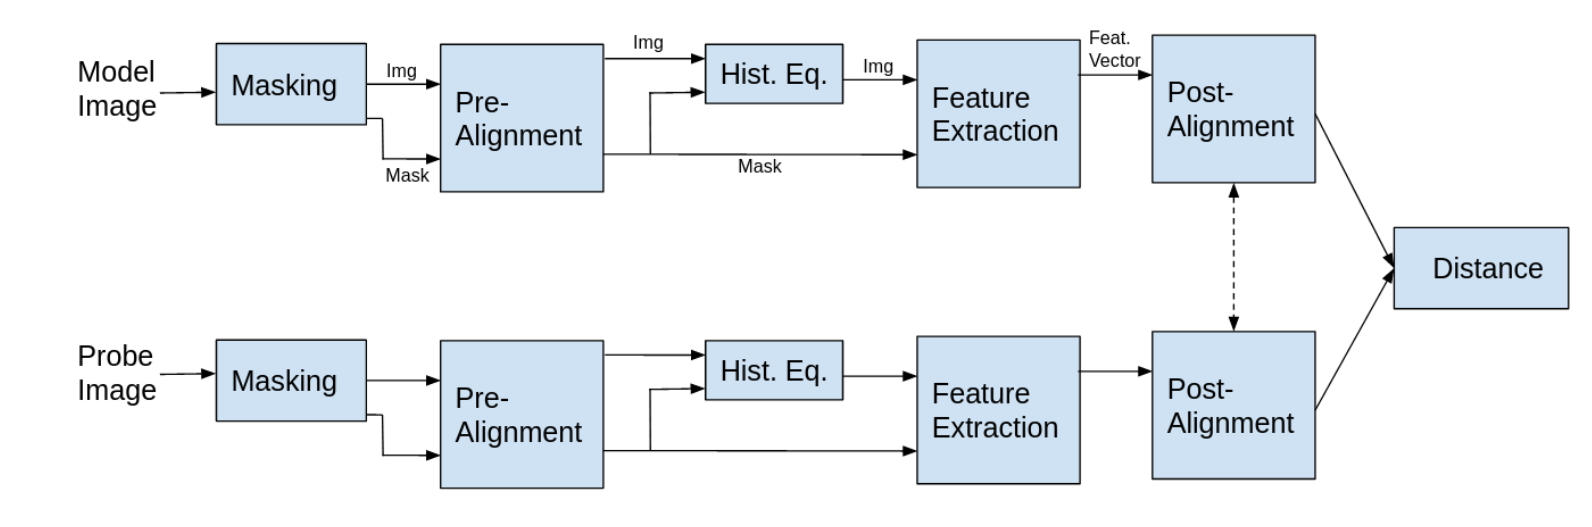
\includegraphics[width=1\linewidth]{latex-img/pipeline_simon.png}
    \caption{Simon's Extraction Pipeline. Compares a single probe image to a model image}
    \label{pipeline_simon}
\end{figure}

Burcu's work on the finger vein authentication project built upon Simon's foundational pipeline, focusing on refining image processing for vein extraction and evaluating different distance calculation methods for authentication. She optimized preprocessing steps, investigated masking and prealignment issues, and tackled reference selection to enhance matching accuracy. A significant part of her contributions involved exploring fuzzy extractors \hyperref[def:Fuzzy_Extractors]{Fuzzy Extractors} to bolster security, conducting a thorough analysis of the dataset to identify and address challenges, and proposing solutions to improve the system's reliability and efficiency.\\

Simon and Burcu explored a variety of function combinations at different stages of the authentication pipeline, aiming to pinpoint the configuration that yields the most favorable outcomes. They utilized the Equal Error Rate (EER) as a benchmark to measure the pipeline's efficacy, focusing on achieving a balance between security and accessibility. This metric, representing the point where the rate of false acceptances (impostor incorrectly granted access) matches the rate of false rejections (legitimate user incorrectly denied), serves as an indicator of the system's reliability and accuracy. The configuration that demonstrated superior performance, leading to the lowest EER and thereby optimizing the process of analyzing and processing images, is showcased in the subsequent figure.

\begin{table}[H]
    \centering
    \caption{EER values for the best pipeline: Edge masking, translation pre-alignment, no pre-processing, no post-
    processing, Miura matching as the post-alignment}
    \begin{tabular}{lc}
    \toprule
    Camera & EER \\
    \midrule
    Camera 1 & 0.041 \\
    Camera 2 & 0.029 \\
    Sum of cameras & 0.030 \\
    \bottomrule
    \end{tabular}
    \label{tab:eervalues_best}
\end{table}

\subsection{Project Overview}

In the progression of our project, building upon the work of Simon and Burcu, we aim to address the inherent variability in biometric data, particularly with finger vein patterns, by considering hash functions. The final objective of the system is to add a hashing step at the end of our established pipeline, prior to the post-alignment phase. The integration of this step serves to enhance security and overall functionality by allowing us to store a hash of each biometric image X in our database, instead of the raw biometric data. Upon receiving a new image Y, we compute hashes for all potential translations of Y, comparing these with the hash of X. Unfortunately, this process is computationally expensive because it requires computing the hash for every possible translation of the image. The purpose of employing a hashing process in this system is multifold:

\begin{itemize}
    \item \textbf{Security}: Hash values can be stored instead of raw biometric data. In the event of a database breach, attackers would find it significantly more challenging to reconstruct the original biometric information from the hashed values due to the one-way nature of hash functions.

    \item \textbf{Consistency}: By focusing on the unique patterns of the biometric trait (like finger-vein patterns) and standardizing how this data is processed and hashed, the system aims to produce consistent hash values for the same individual across different scanning sessions. This is crucial for reliable authentication, ensuring that minor variations in finger placement do not affect the system's ability to recognize the user.

    \item \textbf{Performance}: Hashing biometric data into a compact, fixed-size format facilitates quicker comparison and verification processes. It's more efficient to compare hash values than to perform complex pattern recognition operations on raw biometric images.
\end{itemize}

Traditional hash functions, while pivotal in various data security contexts, generate a unique output for each unique input. This one-to-one mapping means even minor variations in the input — common in biometric data due to natural changes in biological traits or differences in scanning conditions — result in completely different hashes. This sensitivity to input variability poses a challenge in biometric authentication systems, where the goal is to accurately recognize and authenticate an individual despite these natural variations.

Fuzzy hashing stands as a sophisticated solution to this challenge. Unlike traditional hash functions, fuzzy hashing is designed to produce consistent cryptographic keys for inputs that are similar, but not identical. This is particularly advantageous in biometric authentication systems, where it's essential to recognize the same biometric trait across different instances, despite slight variations. The "fuzziness" of this approach allows the system to map these similar inputs to the same or closely related hash values, thereby ensuring that legitimate users are not incorrectly denied access due to minor discrepancies in their biometric data.
Furthermore, the application of fuzzy hashing in our pipeline is instrumental in protecting user privacy. Since the hashed values, rather than raw biometric data, are stored and used for authentication, users' biometric information is safeguarded against potential breaches. Even if hashed values were accessed without authorization, the complexity of fuzzy hashing algorithms makes it extremely challenging to reverse-engineer the original biometric data.\\

The process of our fuzzy hashing algorithm, that we will detail in Section~\ref{sec:Fuzzy Hashing}  begins with a biometric capture, a finger image, which goes through the already developped pipeline~\ref{pipeline_simon} to extract a bitstring. This bitstring undergoes a pre-hashing process, where a subset of significant bits (denoted as vein pixels) is selected based on a permutation keyed by a secure key, resulting in a tuple that significantly reduces the data's dimensionality while preserving its distinguishing features.

Upon generating the fuzzy hash, the next step involves further compressing this hash to prepare it for storage. This compression is achieved through a function, postHash, which maps the tuple to a bitstring of a defined length. The output, essentially a compressed fuzzy hash, exhibits nearly uniform distribution when both the input data and the key are random, enhancing security and storage efficiency.

To further bolster the security of the stored biometric data, this system incorporates \hyperref[def:Fuzzy_Extractors]{Fuzzy Extractors}. The fuzzy extractor framework ensures that even if the stored data is compromised, reconstructing the original biometric data or compromising individual privacy remains computationally infeasible. This is accomplished by generating a secure, random key from the biometric input using a generation process (Gen) and allowing for the reliable reproduction of this key from an approximation of the original input using a reproduction process (Rep), without directly storing the biometric data itself.

In essence, we aim to store the output of the fuzzy extractor, which includes the reproducible cryptographic key and the helper data, instead of the raw biometric data or its direct hash. This method ensures that the stored biometric data is not only compact and efficiently stored but also securely obfuscated, requiring the correct biometric input for any form of decryption or matching to occur.


\section{Introduction}

\subsection{Background}
Authentication is the process of confirming the validity of a claimed identity seeking access to a system or resource. Over decades, authentication mechanisms have evolved from basic password systems in the 1960s to advanced methods such as multifactor authentication by the late 2010s, driven by a persistent commitment to combat evolving security risks while enhancing user convenience\cite{ref1}. Various methods such as password-based authentication, certificate-based authentication, one-time passwords, multifactor authentication, and biometric authentication are employed\cite{ref2}.

Biometric authentication, which involves analyzing unique physical characteristics, is often considered more secure than traditional authentication methods due to the difficulty in duplicating biometric traits. This encompasses technologies such as facial recognition, fingerprint recognition, eye recognition, and voice recognition\cite{ref3}.
However, despite the enhanced security of biometric authentication, it is not immune to exploitation. For instance, fingerprints left on surfaces can be copied, or hackers may obtain images of individuals online to deceive authentication systems.
Choosing the right authentication mechanism requires careful consideration of various factors including the necessary security level, ease of use for users, cost implications for setup and ongoing upkeep, as well as the unique risks and vulnerabilities pertinent to the system or data in question. Typically, the requisite level of security steers the selection process; for example, platforms managing sensitive personal information might mandate the use of robust authentication methods, such as biometric verification. The inherent challenge in deploying such secure systems lies in achieving a delicate equilibrium between high security measures and user convenience. The goal is to create an authentication process that is both seamless and efficient, ensuring that access is granted swiftly and accurately to the rightful user without necessitating multiple attempts, thus maintaining a user-friendly experience while upholding the highest security standards.

While advanced biometric systems typically rely on externally visible physical attributes, finger-vein authentication focuses on internal anatomical features, adding a unique layer of security, as they are less prone to replication or theft compared to external characteristics. Nevertheless, it is important to note that finger-vein authentication does not completely eliminate challenges. Despite its emphasis on internal features, attackers can exploit inherent structures in finger veins, such as common patterns among individuals and predictability in acquired data, which poses risks to the authentication process.\\

In light of these considerations, this project is dedicated to authentication using finger-vein features.
This involves utilizing a specialized scanner equipped with two infrared cameras to capture finger veins from different angles.
The registration process involves capturing an image, termed the model image, while the authentication process involves capturing another image, known as the probe image. These images undergo processing through a pipeline designed to extract and align the finger-vein patterns.
The pipeline outputs a feature vector, which is essentially a bitstring, where 0's represent where there are no finger veins, and 1's show where veins are present.
Following this process, the system evaluates whether the feature vector extracted from the probe image sufficiently matches the feature vector of the model image associated with the individual attempting authentication.

\subsection{Extraction Pipeline}\label{sec:extraction-pipeline}

This project extends the work on optimizing a finger-vein recognition pipeline that has demonstrated the lowest \hyperref[def:EER]{Equal Error Rate (EER)} by incorporating a novel hashing step to process the output of the pipeline. The purpose of integrating \hyperref[def:Hash_Function]{Hash Functions} within this context is multifold, but before delving into hash functions, which are central to our project, it's essential to outline the foundation upon which we have built our advancements. This initial context will provide a clearer understanding of the starting point from which our developments began.\\

Simon Sommerhalder and Burcu Yildiz have both made significant contributions to the system. Simon introduced an innovative approach to the alignment of freshly captured images (probe images) with those stored in the system (model images), ensuring the hashing process (following the alignment of the finger) is based on the unique finger-vein pattern rather than how the finger is positioned on the scanner.

Simon has developped a pipeline (see Figure~\ref{pipeline_simon}) to align finger-vein images, enhancing security by eliminating the need to compare the model and probe images side by side. He organized the pipeline into six clear steps:

\begin{enumerate}
    \item \textbf{Masking}: The first step of the pipeline isolates the finger area in the image. This involves creating a mask that outlines the finger, ensuring that subsequent processing focuses solely on the relevant part of the image.

    \item \textbf{Prealignment}: This step involves adjusting the position and orientation of the finger within the image before extracting vein patterns. It's aimed at roughly aligning the image based on the finger's outline, helping to standardize the position of the finger across different scans.

    \item \textbf{Histogram equalization}: To ensure the images have consistent lighting and contrast, this step adjusts the brightness levels. This makes the vein patterns more distinct and comparable across different images.

    \item \textbf{Feature extraction}: Here, the actual vein patterns are identified and extracted from the image. The process converts the visual image into a digital format that represents the presence or absence of veins at specific locations.

    \item \textbf{Postalignment}: After extracting the vein patterns, this step fine-tunes the alignment of the image. It's based on the vein patterns themselves, ensuring that the comparison between model and probe images is as accurate as possible.

    \item \textbf{Distance Calculation}: The final step involves comparing the feature vector of the probe image with that of the model image. This is done using a specific metric to quantify the similarity between the two, ultimately determining if they match closely enough for authentication to succeed.
\end{enumerate} 

\begin{figure}[!h]
    \centering
    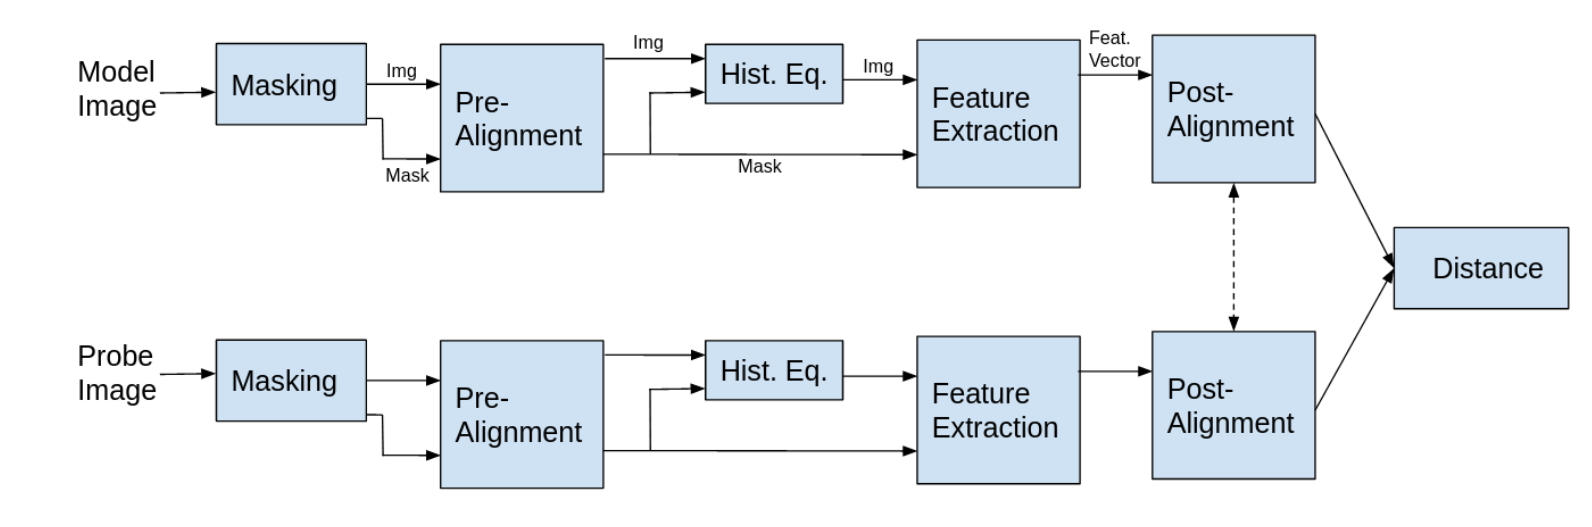
\includegraphics[width=1\linewidth]{latex-img/pipeline_simon.png}
    \caption{Simon's Extraction Pipeline. Compares a single probe image to a model image}
    \label{pipeline_simon}
\end{figure}

Burcu's work on the finger vein authentication project built upon Simon's foundational pipeline, focusing on refining image processing for vein extraction and evaluating different distance calculation methods for authentication. She optimized preprocessing steps, investigated masking and prealignment issues, and tackled reference selection to enhance matching accuracy. A significant part of her contributions involved exploring fuzzy extractors \hyperref[def:Fuzzy_Extractors]{Fuzzy Extractors} to bolster security, conducting a thorough analysis of the dataset to identify and address challenges, and proposing solutions to improve the system's reliability and efficiency.\\

Simon and Burcu explored a variety of function combinations at different stages of the authentication pipeline, aiming to pinpoint the configuration that yields the most favorable outcomes. They utilized the Equal Error Rate (EER) as a benchmark to measure the pipeline's efficacy, focusing on achieving a balance between security and accessibility. This metric, representing the point where the rate of false acceptances (impostor incorrectly granted access) matches the rate of false rejections (legitimate user incorrectly denied), serves as an indicator of the system's reliability and accuracy. The configuration that demonstrated superior performance, leading to the lowest EER and thereby optimizing the process of analyzing and processing images, is showcased in the subsequent figure.

\begin{table}[H]
    \centering
    \caption{EER values for the best pipeline: Edge masking, translation pre-alignment, no pre-processing, no post-
    processing, Miura matching as the post-alignment}
    \begin{tabular}{lc}
    \toprule
    Camera & EER \\
    \midrule
    Camera 1 & 0.041 \\
    Camera 2 & 0.029 \\
    Sum of cameras & 0.030 \\
    \bottomrule
    \end{tabular}
    \label{tab:eervalues_best}
\end{table}

\subsection{Project Overview}

In the progression of our project, building upon the work of Simon and Burcu, we aim to address the inherent variability in biometric data, particularly with finger vein patterns, by considering hash functions. The final objective of the system is to add a hashing step at the end of our established pipeline, prior to the post-alignment phase. The integration of this step serves to enhance security and overall functionality by allowing us to store a hash of each biometric image X in our database, instead of the raw biometric data. Upon receiving a new image Y, we compute hashes for all potential translations of Y, comparing these with the hash of X. Unfortunately, this process is computationally expensive because it requires computing the hash for every possible translation of the image. The purpose of employing a hashing process in this system is multifold:

\begin{itemize}
    \item \textbf{Security}: Hash values can be stored instead of raw biometric data. In the event of a database breach, attackers would find it significantly more challenging to reconstruct the original biometric information from the hashed values due to the one-way nature of hash functions.

    \item \textbf{Consistency}: By focusing on the unique patterns of the biometric trait (like finger-vein patterns) and standardizing how this data is processed and hashed, the system aims to produce consistent hash values for the same individual across different scanning sessions. This is crucial for reliable authentication, ensuring that minor variations in finger placement do not affect the system's ability to recognize the user.

    \item \textbf{Performance}: Hashing biometric data into a compact, fixed-size format facilitates quicker comparison and verification processes. It's more efficient to compare hash values than to perform complex pattern recognition operations on raw biometric images.
\end{itemize}

Traditional hash functions, while pivotal in various data security contexts, generate a unique output for each unique input. This one-to-one mapping means even minor variations in the input — common in biometric data due to natural changes in biological traits or differences in scanning conditions — result in completely different hashes. This sensitivity to input variability poses a challenge in biometric authentication systems, where the goal is to accurately recognize and authenticate an individual despite these natural variations.

Fuzzy hashing stands as a sophisticated solution to this challenge. Unlike traditional hash functions, fuzzy hashing is designed to produce consistent cryptographic keys for inputs that are similar, but not identical. This is particularly advantageous in biometric authentication systems, where it's essential to recognize the same biometric trait across different instances, despite slight variations. The "fuzziness" of this approach allows the system to map these similar inputs to the same or closely related hash values, thereby ensuring that legitimate users are not incorrectly denied access due to minor discrepancies in their biometric data.
Furthermore, the application of fuzzy hashing in our pipeline is instrumental in protecting user privacy. Since the hashed values, rather than raw biometric data, are stored and used for authentication, users' biometric information is safeguarded against potential breaches. Even if hashed values were accessed without authorization, the complexity of fuzzy hashing algorithms makes it extremely challenging to reverse-engineer the original biometric data.\\

The process of our fuzzy hashing algorithm, that we will detail in Section~\ref{sec:Fuzzy Hashing}  begins with a biometric capture, a finger image, which goes through the already developped pipeline~\ref{pipeline_simon} to extract a bitstring. This bitstring undergoes a pre-hashing process, where a subset of significant bits (denoted as vein pixels) is selected based on a permutation keyed by a secure key, resulting in a tuple that significantly reduces the data's dimensionality while preserving its distinguishing features.

Upon generating the fuzzy hash, the next step involves further compressing this hash to prepare it for storage. This compression is achieved through a function, postHash, which maps the tuple to a bitstring of a defined length. The output, essentially a compressed fuzzy hash, exhibits nearly uniform distribution when both the input data and the key are random, enhancing security and storage efficiency.

To further bolster the security of the stored biometric data, this system incorporates \hyperref[def:Fuzzy_Extractors]{Fuzzy Extractors}. The fuzzy extractor framework ensures that even if the stored data is compromised, reconstructing the original biometric data or compromising individual privacy remains computationally infeasible. This is accomplished by generating a secure, random key from the biometric input using a generation process (Gen) and allowing for the reliable reproduction of this key from an approximation of the original input using a reproduction process (Rep), without directly storing the biometric data itself.

In essence, we aim to store the output of the fuzzy extractor, which includes the reproducible cryptographic key and the helper data, instead of the raw biometric data or its direct hash. This method ensures that the stored biometric data is not only compact and efficiently stored but also securely obfuscated, requiring the correct biometric input for any form of decryption or matching to occur.


\section{Biometric Setting}
\label{sec:bio_setting}
This section provides a comprehensive overview of the mathematical and technical aspects involved in fingervein matching, which is essential for comprehending the subsequent discussions in this paper. Additionally, insights into the process of obtaining these equations and statements will be provided, evaluating their relevance and implications within the context of the research. 

\subsection{Biometric Data and Similarity Scores}
\label{Bio_data_sim_scores}
We begin by delving into the representation of the biometric data. Finger images, designated as biometric templates and formated as \(250\)x\(386\), result in \(n\) = \(96'500\) pixels per image. To enhance processing efficiency, these templates are converted into vectors, departing from their original 2-dimension image structure. 

In the biometric context, each finger serves as a biometric subject, with a corresponding biometric capture represented as a bitstring \(X\) of length \(n\). This capture encapsulates the specific vein pixel information extracted from the finger image, while the biometric template serves as a reference mode derived from these images. 

Each of the \(n\) bits of the biometric capture is designated as \(X_1, \ldots, X_n\), with \(X_i\) set to \(1\) if the \(i\)-th bit corresponds to a vein and \(0\) otherwise. We define a random variable as the Hamming Weight of a feature vector \(X\) divided by the total number of bits in the vector \(\left( \frac{\text{HW}(X)}{n} \right)\). The parameter \(p\) is defined as the mean of this random variable.

\begin{equation} \label{eq:p}
    \begin{aligned}
        p = \mathbb{E}\left( \frac{\text{HW}(X)}{n} \right) = Pr\left(X_i = 1\right)
    \end{aligned}
\end{equation}

In the case where \(i\) is a uniformly distributed random index and \(X\) is randomly chosen, the mean (\(p\))\footnote{Throughout this report, experimentally derived variables are denoted with the superscript "obs" (e.g., \(\text{var}^{\text{obs}}\)), while theoretical variables are presented without any superscript.}, along with the variance (\(\sigma²\)) and standard deviation (\(\sigma\)) of the random variable \(\frac{\text{HW}(X)}{n}\) across all images are quantified as follows:

\begin{equation} \label{eq:proba1}
    p^{\text{obs}} = \mathbb{E}\left( \frac{\text{HW}(X)}{n} \right) = 3.29\%
\end{equation}

\begin{equation} \label{eq:proba2}
    \sigma^{\text{obs}} = \sqrt{\mathbb{E} \left[ \left( \frac{\text{HW}(X)}{n} - p^{\text{obs}} \right)^2 \right]} \approx 4.69 \times 10^{-3}
\end{equation}


\begin{equation} \label{eq:proba3}
    (\sigma^{\text{obs}})² = \mathbb{V}\left( \frac{\text{HW}(X)}{n} \right)  \approx 2.20 \times 10^{-5}
\end{equation}

where \( \sigma \) and \( \sigma^2 \) represent the standard deviation and variance of the random variable \(\frac{\text{HW}(X)}{n}\) respectively.

In biometric authentication and identification, the uniqueness of each biometric capture is encoded in its bits. The objective revolves around discerning the similarity between two biometric captures to verify or identify two individuals. Therefore, the scoring mechansim plays a crucial role in quantatively determining the similarity between biometric captures. This similarity score holds significance in verifying the identity of an individual (authentication) or identifying potential matches in a database (identification). A higher score indicates a greater ressemblance between captures, while a lower score suggests less similarity. This scoring mechanism is indispensable for ensuring the accuracy and reliability of biometric systems. The score of (\(X\), \(Y\)) is computed as

\begin{equation} \label{eq:score}
    \begin{aligned}
        Score(X, Y) &= \frac{HW(X \land Y)}{HW(X) + HW(Y)}\\
        &= \frac{1}{2}-\frac{1}{2}\frac{d_H(X, Y)}{HW(X) + HW(Y)}
    \end{aligned}
\end{equation}

where \(HW\) denotes the \hyperref[def:Hamming Weight]{Hamming Weight} and \(d_H\) the \hyperref[def:Hamming Distance]{Hamming Distance}. 

In conjunction with the scoring mechanism, Miura matching emerges as a specialized technique for comparing biometric samples. This method entails determining an optimal offset translation, denoted as \(d_X\) and \(d_Y\), between two biometric samples to align their features for comparison, thereby compensating for differences in positioning or orientation. The alignment process maximizes the similarity score, defined as:

\[Score = \text{Score}(d_X \cdot X, d_Y \cdot Y)\]

Once the optimal offsets, \(d_X\) and \(d_Y\), are determined, they are applied to the original samples for alignment. This results in the calculated aligned positions, denoted as \(\bar{X}\) and \(\bar{Y}\), such that:

\[\bar{X} = d_X \cdot X\]
\[\bar{Y} = d_Y \cdot Y\]

Miura matching and the scoring mechanism are interconnected components, where Miura matching facilitates the computation of the score, thereby offering insights into the similarity between biometric captures and enhancing the reliability of matching algorithms.

The probability of the \(i\)-th pixel of two captures not being the same after applying the optimal offset translations depends on the distribution of \((\bar{X}, \bar{Y})\), and is denoted as \(\delta\). We define the random variable as the normalized Hamming distance between two feature vectors \(\left( \frac{d_H(\bar{X}, \bar{Y})}{n} \right)\). The parameter \(\delta\) is defined as the mean of this random variable, and we additionally define the standard deviation and the variance of this random variable, as shown in the following figures.



\begin{equation} \label{eq:delta}
    \begin{aligned}
        \delta = \mathbb{E}\left( \frac{d_H(\bar{X}, \bar{Y})}{n} \right)
    \end{aligned}
\end{equation}

\begin{equation}
    \begin{aligned}
        \sigma_{\delta} = {\sigma}\left( \frac{d_H(\bar{X}, \bar{Y})}{n} \right)
    \end{aligned}
\end{equation}

\begin{equation}
    \begin{aligned}
        \sigma^2_{\delta} = {Var}\left( \frac{d_H(\bar{X}, \bar{Y})}{n} \right)
    \end{aligned}
\end{equation}

Distinguishing between the types of distributions associated with the two captures is crucial. When both captures originate from the same biometric subject, it is referred to as \(\delta_{\text{same}}\). Conversely, if the captures are from different subjects, it is labeled as \(\delta_{\text{diff}}\). Additionally, when \(\bar{X}\) and \(\bar{Y}\) consist of \(2n\) independent random bits with an expected value of \(p\) and no optimal offset is applied, it is classified as \(\delta_{\text{indep}}\). In this scenario, \(\delta_{\text{indep}}^{\text{obs}} = 2p(1-p) = 6.4\%\). As developed in Section~\ref{sec:delta}, the experimental results produce the following figures:

\begin{table}[H]
    \centering
    \renewcommand{\arraystretch}{1.25}
    \begin{tabular}{|c|c|c|c|}
        \hline
        & \textbf{\(\delta^{\text{obs}}\)} & \textbf{\({\sigma^2_{\delta}}^{\text{obs}}\)} & \textbf{\(\sigma_{\delta}^{\text{obs}}\)} \\
        \hline
        \text{Same-Finger Distribution} & 4.55\% & \(1.06 \times 10^{-4}\) & \(1.03 \times 10^{-2}\) \\
        \hline
        \text{Different-Finger Distribution} & 5.99\% & \(4.58 \times 10^{-5}\) & \(6.76 \times 10^{-3}\) \\
        \hline
    \end{tabular}
    \caption{Comparison of Distributions: Mean, Variance, and Standard Deviation of \(\frac{d_H(\bar{X}, \bar{Y})}{n}\) when both captures originate from the same finger and from different fingers}
\end{table}


Utilizing \(p\) (\ref{eq:p}) and $\delta$ (\ref{eq:delta}), the joint distribution for (\(\bar{X}_j\), \(\bar{Y}_j\)) across \(j\) random instances is derived:

\begin{table}[H]
    \centering
    \renewcommand{\arraystretch}{1.5}
    \begin{tabular}{|c|c|c|}
        \hline
        & $\bar{Y}_i = 0$ & $\bar{Y}_i = 1$\\
        \hline
        $\bar{X}_i = 0$ & $1 - p - \frac{\delta}{2}$ & $\frac{\delta}{2}$\\
        \hline
        $\bar{X}_i = 1$ & $\frac{\delta}{2}$ & $p - \frac{\delta}{2}$\\
        \hline
    \end{tabular}
    \caption{Joint Distribution of ($\bar{X}_j$, $\bar{Y}_j$) for Random Instances}
    \label{tab:joint_distribution}
\end{table}

\subsection{Experimental Derivation of the Probability \(p\)}

In order to derive the probability that a distributed random pixel is a vein, \(p\) (\ref{eq:p}), a dataset of 20 unique individuals was utilized. Each individual contributed images of both right and left index/middle fingers, with 5 trials per finger, captured using 2 different cameras. This methodology resulted in a comprehensive dataset of 800 images. Following the approach in Section~\ref{sec:extraction-pipeline}, Simon's optimal pipeline was implemented to extract the feature vectors from each image in the dataset (refer to Figure~\ref{pipeline_simon}). Subsequently, statistical analysis was performed on these feature vectors to gain insights into vein patterns, building on the preliminary work by Burcu. It's important to note that the calculation of the probability \(p\) does not take into account any postalignment method, like Miura Matching, even though the code might seem like it does.

We have carried out this analysis by implementing an algorithm which processes the dataset's feature vectors, performing two main functions:
\begin{enumerate}
    \item For each pixel position, it updates a \textit{veins[i]} array, which accumulates detections of veins across all images for each camera \(i={1,2}\).
    \item It maintains a count of the number of images analyzed per camera \(i={1,2}\) in a \textit{image\_count[i]} array.
\end{enumerate}

Following the processing of all feature vectors, the algorithm computes the probability of a pixel being part of a vein by dividing the aggregated vein detections by the total number of images analyzed, across both cameras. Visual representations were generated to illustrate the distribution of detected vein pixels for each camera individually and for the combined data from both cameras.
\newpage
\begin{enumerate}
    \item \textbf{Camera 1 and Camera 2 distribution}: The following histograms showcase the frequency distribution of vein pixels detected in images captured by Camera 1 and 2 individually, with a Gaussian fit overlaid to highlight the data's normal distribution trend.

    \begin{figure}[H]
        \centering
        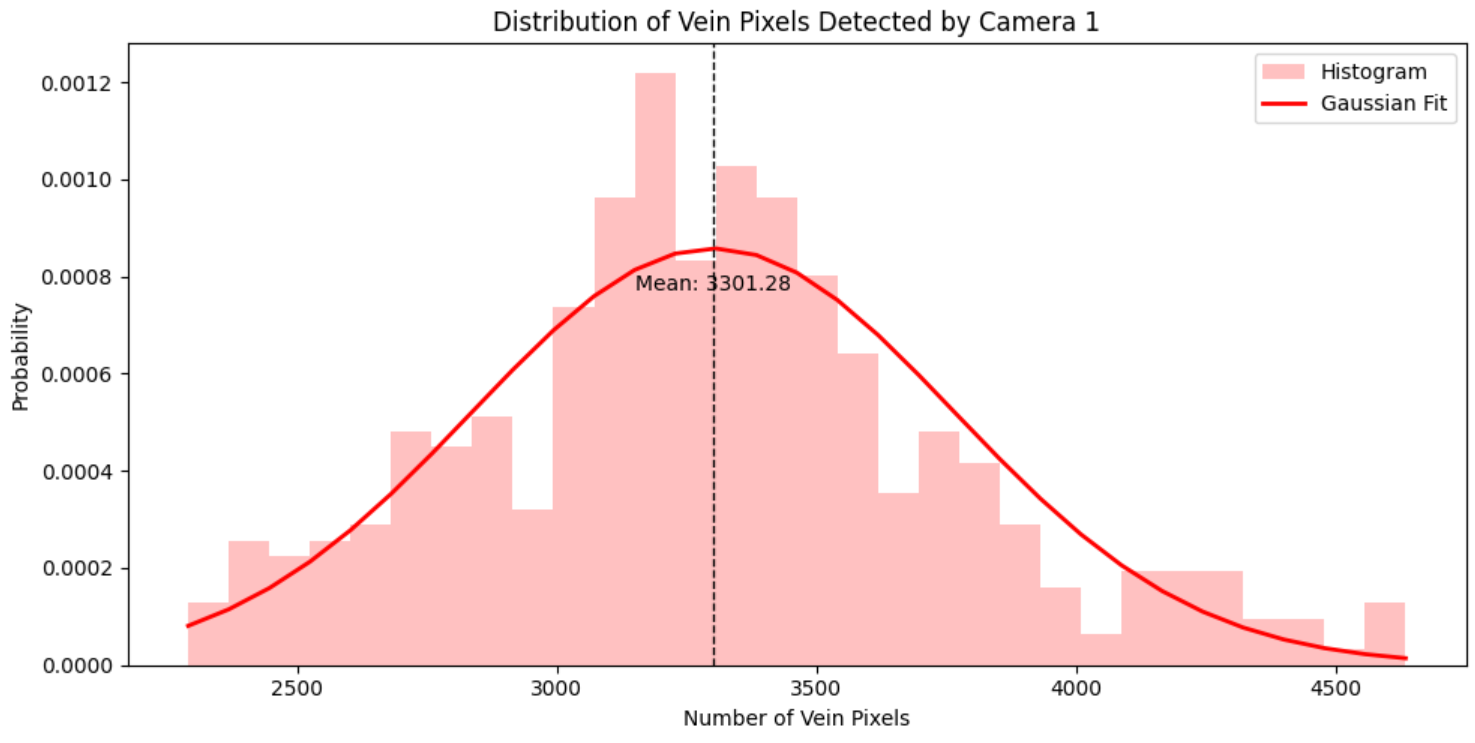
\includegraphics[width=1\linewidth]{latex-img/distribution_veins_cam1.png}
        \caption{Vein Pixel Distribution Analysis Using Camera 1: Histogram Representation with Gaussian Fit Overlay with \(X_i \sim \mathcal{N}(3301.28, 216433.17)\)}
        \label{distribution_veins_cam1}
    \end{figure}

    \begin{figure}[H]
        \centering
        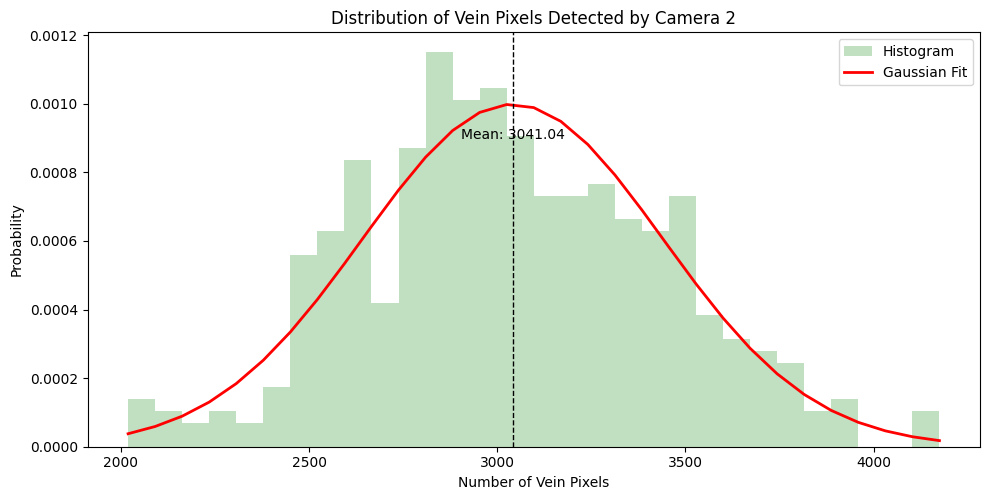
\includegraphics[width=1\linewidth]{latex-img/distribution_veins_cam2.png}
        \caption{Vein Pixel Distribution Analysis Using Camera 2: Histogram Representation with Gaussian Fit Overlay \(X_i \sim \mathcal{N}(3041.04, 159577.13)\)}
        \label{distribution_veins_cam2}
    \end{figure}
 
    \newpage
    \item \textbf{Combined Cameras Distribution}: To understand the aggregate behavior of vein detection across both cameras, the data was merged, generating a comprehensive histogram with a Gaussian fit.

    \begin{figure}[H]
        \centering
        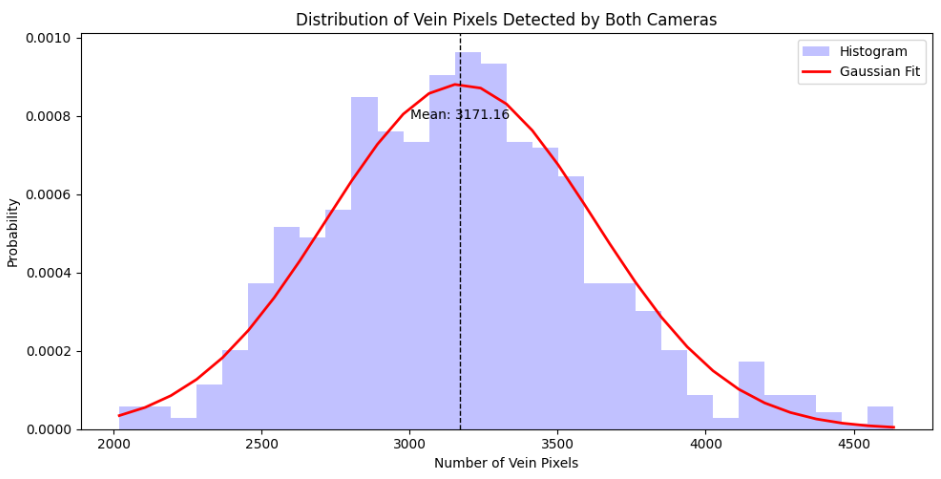
\includegraphics[width=1\linewidth]{latex-img/distribution_veins_bothcams.png}
        \caption{Aggregate Vein Pixel Distribution Analysis: Combined Histogram and Gaussian Fit from Both Cameras \(X_i \sim \mathcal{N}(3171.16, 204935.79)\)}
        \label{distribution_veins_bothcams}
    \end{figure}

\end{enumerate}

Concluding the analysis of the vein pixel distribution across different camera captures and their aggregate dataset, the average probability \(p\) that a given pixel corresponds to a vein was computed. This involved summing up all vein-identifying pixels within the datasets for Camera 1, Camera 2, and the combined dataset. Subsequently, this sum was divided by the total number of pixels processed, multiplying the count of images by the total pixels per image, to ascertain the average likelihood \(p\) that any randomly selected pixel is part of a vein pattern.

The findings from this analysis revealed the following probabilities:
\begin{enumerate}
    \item For Camera 1, the probability \(p^{obs} = \mathbb{E}\left( \frac{\text{HW}(X)}{n} \right)\) was calculated to be \(0.034\), indicating a \(3.42\)\% chance that any given pixel in images from Camera 1 represents a vein.

    \item For Camera 2, the probability \(p^{obs} = \mathbb{E}\left( \frac{\text{HW}(X)}{n} \right)\) was slightly lower at \(0.032\), translating to a \(3.15\)\% chance for vein representation in its images.

    \item When considering the datasets from Both Cameras combined, the probability \(p^{obs} = \mathbb{E}\left( \frac{\text{HW}(X)}{n} \right)\) averaged out to \(0.0329\), suggesting a \(3.29\)\% likelihood of a pixel depicting a vein across the entire dataset. Moreover, the variance (\( \sigma^{2}_p \)) and the standard deviation (\( \sigma_p \)) of the random variable \(\frac{\text{HW}(X)}{n}\) provide insights into the the random variable's spread and consistency. The observed variance is low at approximately \( 2.20 \times 10^{-5} \), indicating minimal fluctuation in the random variables' values among different feature vectors. This suggests that the feature extraction method is highly reliable and consistent across different images. Furthermore, the standard deviation, calculated as approximately \( 4.69 \times 10^{-3} \), reinforces the idea of minimal dispersion around the mean probability (\(p\)) of detecting a vein. 
    
\end{enumerate}

\newpage
\subsection{Experimental Derivation of the Probabilities \(\delta_{\text{same}}, \delta_{\text{diff}}, \delta_{\text{indep}}\)}
\label{sec:delta}

To assess the probability that the i-th pixel of two captures diverges after applying the optimal offset translations \( d_X \) and \( d_Y \) (Equation (\ref{eq:delta})), we undertake additional experimental analysis. This investigation continues to utilize the same dataset comprising 20 distinct individuals. Here, the post-alignment process, specifically Miura Matching, is included in our examination as the calculation formula integrates this step. As detailed in Section~\ref{Bio_data_sim_scores}, our objective is to evaluate three distinct delta values: \(\delta_{\text{same}}, \delta_{\text{diff}}, \delta_{\text{indep}}\). The computation of \( \delta_{\text{indep}} \) is relatively straightforward, having determined the value of \( p \). The formula for \( \delta_{\text{indep}} \) relies solely on \( p \), allowing us to express it as:

\[ \delta_{\text{indep}}^{obs} = 2p^{obs}(1 - p^{obs}) = 2 \times 0.033 \times (1 - 0.033) \approx 6.4\% \]

This result provides an estimated \(6.4\)\% independent delta value.

To accurately evaluate \( \delta_{\text{same}} \) and \( \delta_{\text{diff}} \), a meticulous procedure was executed on our dataset, which involves 20 unique individuals, each having multiple biometric captures. Below is an outline of the methodology applied:

\begin{enumerate}
    \item \textbf{Pairwise Comparison}: For each individual, we compared every biometric capture to every other capture within the dataset, applying the Hamming distance metric to compute the normalized distances.
    \item \textbf{Statistical Analysis}: We organized the resulting distances into two distinct categories:
    \begin{itemize}
        \item Intra-individual distances, where captures from the same individual (same finger images) were compared, forming the first group.
        \item Inter-individual distances, comprising comparisons between biometric captures from different individuals, forming the second group.
    \end{itemize}
    \newpage
    \item \textbf{Probability Computation}:
    \begin{itemize}
        \item For \( \delta_{\text{same}} \), we calculated the average normalized distances from intra-individual comparisons. This analysis provided the following results, quantifying the observed differences between captures from the same individual after alignment:

        \[ \delta_{\text{same}}^{obs} \approx 4.55\% \]
        \[ \sigma_{\delta_{same}} \approx 1.03 \times 10^{-2} \]
        \[ \sigma²_{\delta_{same}} \approx 1.06 \times 10^{-4} \]

        \begin{figure}[H]
            \centering
            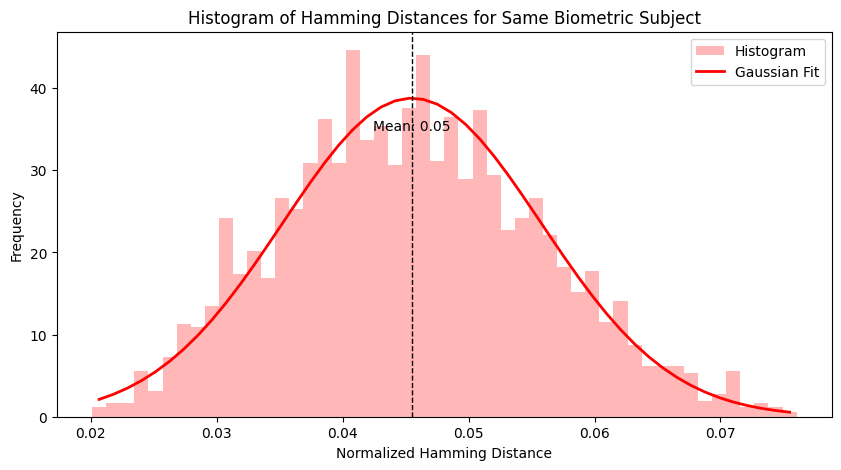
\includegraphics[width=0.7\linewidth]{latex-img/delta_same.png}
            \caption{Frequency Distribution of Normalized Hamming Distances for Identical Biometric Samples with Alignment \(\delta_{same} \sim \mathcal{N}(0.045, 0.000106)\)}
            \label{delta_same}
        \end{figure}
        
        \item For \( \delta_{\text{diff}} \), we performed a similar averaging of the normalized distances from the inter-individual comparisons, which furnished us with the following results for observing a difference between captures from the different individuals after alignment:

        \[ \delta_{\text{diff}}^{obs} \approx 5.99\% \]
        \[ \sigma_{\delta_{diff}} \approx 6.76 \times 10^{-3} \]
        \[ \sigma²_{\delta_{diff}} \approx 4.58 \times 10^{-5} \]

        \begin{figure}[H]
            \centering
            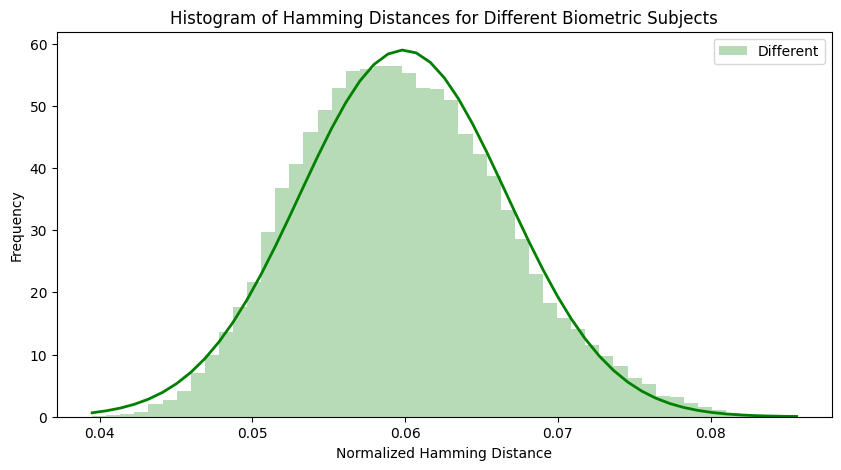
\includegraphics[width=0.7\linewidth]{latex-img/delta_diff.png}
            \caption{Frequency Distribution of Normalized Hamming Distances for Different Biometric Samples with Alignment \(\delta_{diff} \sim \mathcal{N}(0.0599, 0.0000458)\)}
            \label{delta_diff}
        \end{figure}
    \end{itemize}
\end{enumerate}

The joint probability distribution presented in Table \ref{tab:joint_distribution} represents the relationship between the variables \(\bar{X}_i\) and \(\bar{Y}_i\), which compare the i-th bit of two biometric samples. The parameter \(p\) denotes the probability of a bit being '1', and by complement, \(1-p\) signifies the probability of a bit being '0'. The parameter \(\delta\) encapsulates the probability that the two bits are not identical, which can occur due to various sources of error in biometric comparison. 

In Table \ref{tab:joint_distribution}, we explain each entry:

\begin{itemize}
    \item By utilizing the previously determined value of $\delta$, we can infer the probabilities \(P[\bar{X}_i = 1, \bar{Y}_i = 0]\) and \(P[\bar{X}_i = 0, \bar{Y}_i = 1]\) as follows: 
    \begin{equation*}
        \begin{aligned}
            \delta = P[\bar{X}_i \neq \bar{Y}_i] = P[\bar{X}_i = 1, \bar{Y}_i = 0] + P[\bar{X}_i = 0, \bar{Y}_i = 1]
        \end{aligned}
    \end{equation*}
    Hence we have:
    \begin{equation*}
        \begin{aligned}
            P[\bar{X}_i = 1, \bar{Y}_i = 0] = P[\bar{X}_i = 0, \bar{Y}_i = 1] = \frac{\delta}{2}
        \end{aligned}
    \end{equation*}
    \item To determine the probability\(P[\bar{X}_i = 0, \bar{Y}_i = 0]\), we consider the following relationships and utilize the law of total probability:
    \begin{equation*}
        \begin{aligned}
            P[\bar{X}_i = 0] = 1-p = P[\bar{X}_i = 0, \bar{Y}_i = 0] + P[\bar{X}_i = 0, \bar{Y}_i = 1]
        \end{aligned}
    \end{equation*} 
    \begin{equation*}
        \begin{aligned}
            P[\bar{Y}_i = 0] = 1-p = P[\bar{X}_i = 0, \bar{Y}_i = 0] + P[\bar{X}_i = 1, \bar{Y}_i = 0]
        \end{aligned}
    \end{equation*} 
    
    By solving these equations, we can derive the probability of interest, \\\(P[\bar{X}_i = 0, \bar{Y}_i = 0]\), and hence infer the previously obtained values for \\\(P[\bar{X}_i = 1, \bar{Y}_i = 0]\) and \(P[\bar{X}_i = 0, \bar{Y}_i = 1]\):
    \[ P[\bar{X}_i = 0, \bar{Y}_i = 0] = 1-p - \frac{\delta}{2} \] 

    \item The probability \(P[\bar{X}_i = 1, \bar{Y}_i = 1]\) is derived by 
    \[P[\bar{X}_i = 1, \bar{Y}_i = 1] = 1 - P[\bar{X}_i = 0, \bar{Y}_i = 0] = p-\frac{\delta}{2}\]

\end{itemize}

Utilizing \(\delta_{same}^{obs}\), \(\delta_{diff}^{obs}\) and \(\delta_{indep}^{obs}\), we can determine the corresponding probabilities presented in Table \ref{tab:joint_distribution}. This gives us the following figures:

\begin{table}[H]
    \centering
    \renewcommand{\arraystretch}{1.5}
    \begin{tabular}{|c|c|c|}
        \hline
        & $\bar{Y}_i = 0$ & $\bar{Y}_i = 1$\\
        \hline
        $\bar{X}_i = 0$ & $1 - p - \frac{\delta_{indep}^{obs}}{2} = 93.5\% $ & $\frac{\delta_{indep}^{obs}}{2} = 3.2\%$\\
        \hline
        $\bar{X}_i = 1$ & $\frac{\delta_{indep}^{obs}}{2} = 3.2\% $ & $p - \frac{\delta_{indep}^{obs}}{2} = 0.1\%$\\
        \hline
    \end{tabular}
    \caption{Joint Distribution of ($\bar{X}_j$, $\bar{Y}_j$) for \(X\) and \(Y\) made up of \(2n\) independent random bits of expected value \(p\)}
    \label{tab:joint_distribution_deltaindep}
\end{table}


\begin{table}[H]
    \centering
    \renewcommand{\arraystretch}{1.5}
    \begin{tabular}{|c|c|c|}
        \hline
        & $\bar{Y}_i = 0$ & $\bar{Y}_i = 1$\\
        \hline
        $\bar{X}_i = 0$ & $1 - p - \frac{\delta_{same}^{obs}}{2} = 94.4\% $ & $\frac{\delta_{same}^{obs}}{2} = 2.3\%$\\
        \hline
        $\bar{X}_i = 1$ & $\frac{\delta_{same}^{obs}}{2} = 2.3\%$ & $p - \frac{\delta_{same}^{obs}}{2} = 1\%$\\
        \hline
    \end{tabular}
    \caption{Joint Distribution of ($\bar{X}_j$, $\bar{Y}_j$) for \(X\) and \(Y\)  Originating from the Same Biometric Subject}
    \label{tab:joint_distribution_deltasame}
\end{table}

\begin{table}[H]
    \centering
    \renewcommand{\arraystretch}{1.5}
    \begin{tabular}{|c|c|c|}
        \hline
        & $\bar{Y}_i = 0$ & $\bar{Y}_i = 1$\\
        \hline
        $\bar{X}_i = 0$ & $1 - p - \frac{\delta_{diff}^{obs}}{2} = 93.7\% $ & $\frac{\delta_{diff}^{obs}}{2} = 3\%$\\
        \hline
        $\bar{X}_i = 1$ & $\frac{\delta_{diff}^{obs}}{2} = 3\%$ & $p - \frac{\delta_{diff}^{obs}}{2} = 0.3\%$\\
        \hline
    \end{tabular}
    \caption{Joint Distribution of ($\bar{X}_j$, $\bar{Y}_j$) for \(X\) and \(Y\) Originating from Different Biometric Subject}
    \label{tab:joint_distribution_deltadiff}
\end{table}









\section{Introduction}

\subsection{Background}
Authentication is the process of confirming the validity of a claimed identity seeking access to a system or resource. Over decades, authentication mechanisms have evolved from basic password systems in the 1960s to advanced methods such as multifactor authentication by the late 2010s, driven by a persistent commitment to combat evolving security risks while enhancing user convenience\cite{ref1}. Various methods such as password-based authentication, certificate-based authentication, one-time passwords, multifactor authentication, and biometric authentication are employed\cite{ref2}.

Biometric authentication, which involves analyzing unique physical characteristics, is often considered more secure than traditional authentication methods due to the difficulty in duplicating biometric traits. This encompasses technologies such as facial recognition, fingerprint recognition, eye recognition, and voice recognition\cite{ref3}.
However, despite the enhanced security of biometric authentication, it is not immune to exploitation. For instance, fingerprints left on surfaces can be copied, or hackers may obtain images of individuals online to deceive authentication systems.
Choosing the right authentication mechanism requires careful consideration of various factors including the necessary security level, ease of use for users, cost implications for setup and ongoing upkeep, as well as the unique risks and vulnerabilities pertinent to the system or data in question. Typically, the requisite level of security steers the selection process; for example, platforms managing sensitive personal information might mandate the use of robust authentication methods, such as biometric verification. The inherent challenge in deploying such secure systems lies in achieving a delicate equilibrium between high security measures and user convenience. The goal is to create an authentication process that is both seamless and efficient, ensuring that access is granted swiftly and accurately to the rightful user without necessitating multiple attempts, thus maintaining a user-friendly experience while upholding the highest security standards.

While advanced biometric systems typically rely on externally visible physical attributes, finger-vein authentication focuses on internal anatomical features, adding a unique layer of security, as they are less prone to replication or theft compared to external characteristics. Nevertheless, it is important to note that finger-vein authentication does not completely eliminate challenges. Despite its emphasis on internal features, attackers can exploit inherent structures in finger veins, such as common patterns among individuals and predictability in acquired data, which poses risks to the authentication process.\\

In light of these considerations, this project is dedicated to authentication using finger-vein features.
This involves utilizing a specialized scanner equipped with two infrared cameras to capture finger veins from different angles.
The registration process involves capturing an image, termed the model image, while the authentication process involves capturing another image, known as the probe image. These images undergo processing through a pipeline designed to extract and align the finger-vein patterns.
The pipeline outputs a feature vector, which is essentially a bitstring, where 0's represent where there are no finger veins, and 1's show where veins are present.
Following this process, the system evaluates whether the feature vector extracted from the probe image sufficiently matches the feature vector of the model image associated with the individual attempting authentication.

\subsection{Extraction Pipeline}\label{sec:extraction-pipeline}

This project extends the work on optimizing a finger-vein recognition pipeline that has demonstrated the lowest \hyperref[def:EER]{Equal Error Rate (EER)} by incorporating a novel hashing step to process the output of the pipeline. The purpose of integrating \hyperref[def:Hash_Function]{Hash Functions} within this context is multifold, but before delving into hash functions, which are central to our project, it's essential to outline the foundation upon which we have built our advancements. This initial context will provide a clearer understanding of the starting point from which our developments began.\\

Simon Sommerhalder and Burcu Yildiz have both made significant contributions to the system. Simon introduced an innovative approach to the alignment of freshly captured images (probe images) with those stored in the system (model images), ensuring the hashing process (following the alignment of the finger) is based on the unique finger-vein pattern rather than how the finger is positioned on the scanner.

Simon has developped a pipeline (see Figure~\ref{pipeline_simon}) to align finger-vein images, enhancing security by eliminating the need to compare the model and probe images side by side. He organized the pipeline into six clear steps:

\begin{enumerate}
    \item \textbf{Masking}: The first step of the pipeline isolates the finger area in the image. This involves creating a mask that outlines the finger, ensuring that subsequent processing focuses solely on the relevant part of the image.

    \item \textbf{Prealignment}: This step involves adjusting the position and orientation of the finger within the image before extracting vein patterns. It's aimed at roughly aligning the image based on the finger's outline, helping to standardize the position of the finger across different scans.

    \item \textbf{Histogram equalization}: To ensure the images have consistent lighting and contrast, this step adjusts the brightness levels. This makes the vein patterns more distinct and comparable across different images.

    \item \textbf{Feature extraction}: Here, the actual vein patterns are identified and extracted from the image. The process converts the visual image into a digital format that represents the presence or absence of veins at specific locations.

    \item \textbf{Postalignment}: After extracting the vein patterns, this step fine-tunes the alignment of the image. It's based on the vein patterns themselves, ensuring that the comparison between model and probe images is as accurate as possible.

    \item \textbf{Distance Calculation}: The final step involves comparing the feature vector of the probe image with that of the model image. This is done using a specific metric to quantify the similarity between the two, ultimately determining if they match closely enough for authentication to succeed.
\end{enumerate} 

\begin{figure}[!h]
    \centering
    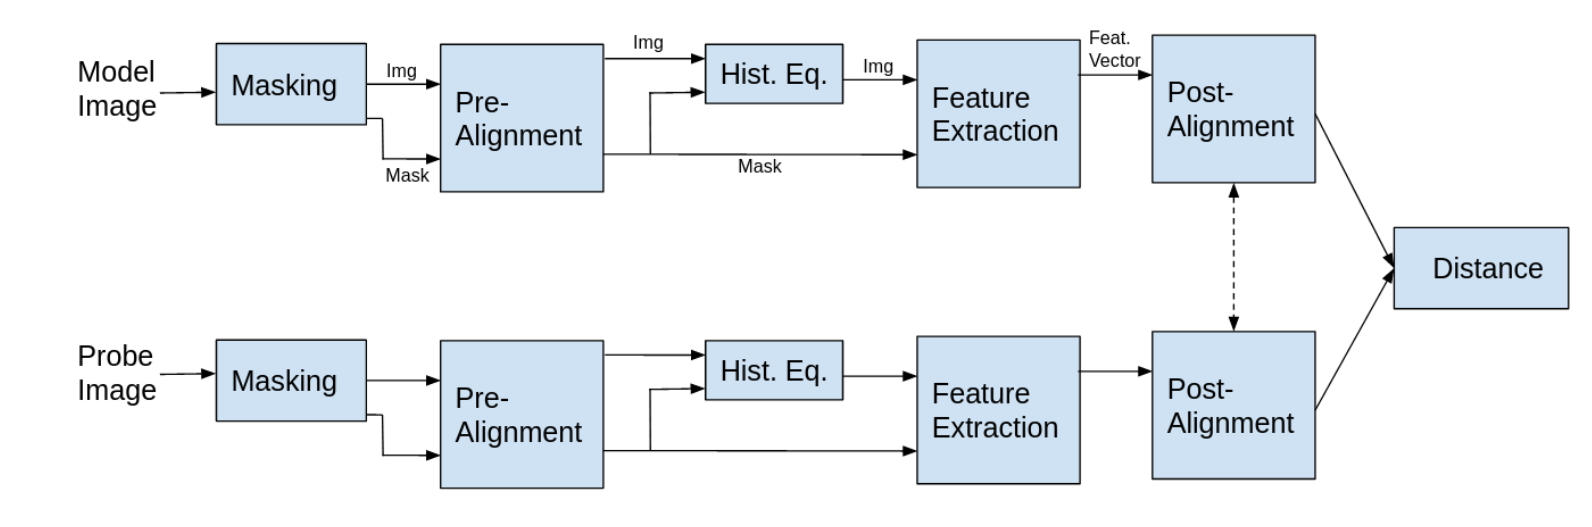
\includegraphics[width=1\linewidth]{latex-img/pipeline_simon.png}
    \caption{Simon's Extraction Pipeline. Compares a single probe image to a model image}
    \label{pipeline_simon}
\end{figure}

Burcu's work on the finger vein authentication project built upon Simon's foundational pipeline, focusing on refining image processing for vein extraction and evaluating different distance calculation methods for authentication. She optimized preprocessing steps, investigated masking and prealignment issues, and tackled reference selection to enhance matching accuracy. A significant part of her contributions involved exploring fuzzy extractors \hyperref[def:Fuzzy_Extractors]{Fuzzy Extractors} to bolster security, conducting a thorough analysis of the dataset to identify and address challenges, and proposing solutions to improve the system's reliability and efficiency.\\

Simon and Burcu explored a variety of function combinations at different stages of the authentication pipeline, aiming to pinpoint the configuration that yields the most favorable outcomes. They utilized the Equal Error Rate (EER) as a benchmark to measure the pipeline's efficacy, focusing on achieving a balance between security and accessibility. This metric, representing the point where the rate of false acceptances (impostor incorrectly granted access) matches the rate of false rejections (legitimate user incorrectly denied), serves as an indicator of the system's reliability and accuracy. The configuration that demonstrated superior performance, leading to the lowest EER and thereby optimizing the process of analyzing and processing images, is showcased in the subsequent figure.

\begin{table}[H]
    \centering
    \caption{EER values for the best pipeline: Edge masking, translation pre-alignment, no pre-processing, no post-
    processing, Miura matching as the post-alignment}
    \begin{tabular}{lc}
    \toprule
    Camera & EER \\
    \midrule
    Camera 1 & 0.041 \\
    Camera 2 & 0.029 \\
    Sum of cameras & 0.030 \\
    \bottomrule
    \end{tabular}
    \label{tab:eervalues_best}
\end{table}

\subsection{Project Overview}

In the progression of our project, building upon the work of Simon and Burcu, we aim to address the inherent variability in biometric data, particularly with finger vein patterns, by considering hash functions. The final objective of the system is to add a hashing step at the end of our established pipeline, prior to the post-alignment phase. The integration of this step serves to enhance security and overall functionality by allowing us to store a hash of each biometric image X in our database, instead of the raw biometric data. Upon receiving a new image Y, we compute hashes for all potential translations of Y, comparing these with the hash of X. Unfortunately, this process is computationally expensive because it requires computing the hash for every possible translation of the image. The purpose of employing a hashing process in this system is multifold:

\begin{itemize}
    \item \textbf{Security}: Hash values can be stored instead of raw biometric data. In the event of a database breach, attackers would find it significantly more challenging to reconstruct the original biometric information from the hashed values due to the one-way nature of hash functions.

    \item \textbf{Consistency}: By focusing on the unique patterns of the biometric trait (like finger-vein patterns) and standardizing how this data is processed and hashed, the system aims to produce consistent hash values for the same individual across different scanning sessions. This is crucial for reliable authentication, ensuring that minor variations in finger placement do not affect the system's ability to recognize the user.

    \item \textbf{Performance}: Hashing biometric data into a compact, fixed-size format facilitates quicker comparison and verification processes. It's more efficient to compare hash values than to perform complex pattern recognition operations on raw biometric images.
\end{itemize}

Traditional hash functions, while pivotal in various data security contexts, generate a unique output for each unique input. This one-to-one mapping means even minor variations in the input — common in biometric data due to natural changes in biological traits or differences in scanning conditions — result in completely different hashes. This sensitivity to input variability poses a challenge in biometric authentication systems, where the goal is to accurately recognize and authenticate an individual despite these natural variations.

Fuzzy hashing stands as a sophisticated solution to this challenge. Unlike traditional hash functions, fuzzy hashing is designed to produce consistent cryptographic keys for inputs that are similar, but not identical. This is particularly advantageous in biometric authentication systems, where it's essential to recognize the same biometric trait across different instances, despite slight variations. The "fuzziness" of this approach allows the system to map these similar inputs to the same or closely related hash values, thereby ensuring that legitimate users are not incorrectly denied access due to minor discrepancies in their biometric data.
Furthermore, the application of fuzzy hashing in our pipeline is instrumental in protecting user privacy. Since the hashed values, rather than raw biometric data, are stored and used for authentication, users' biometric information is safeguarded against potential breaches. Even if hashed values were accessed without authorization, the complexity of fuzzy hashing algorithms makes it extremely challenging to reverse-engineer the original biometric data.\\

The process of our fuzzy hashing algorithm, that we will detail in Section~\ref{sec:Fuzzy Hashing}  begins with a biometric capture, a finger image, which goes through the already developped pipeline~\ref{pipeline_simon} to extract a bitstring. This bitstring undergoes a pre-hashing process, where a subset of significant bits (denoted as vein pixels) is selected based on a permutation keyed by a secure key, resulting in a tuple that significantly reduces the data's dimensionality while preserving its distinguishing features.

Upon generating the fuzzy hash, the next step involves further compressing this hash to prepare it for storage. This compression is achieved through a function, postHash, which maps the tuple to a bitstring of a defined length. The output, essentially a compressed fuzzy hash, exhibits nearly uniform distribution when both the input data and the key are random, enhancing security and storage efficiency.

To further bolster the security of the stored biometric data, this system incorporates \hyperref[def:Fuzzy_Extractors]{Fuzzy Extractors}. The fuzzy extractor framework ensures that even if the stored data is compromised, reconstructing the original biometric data or compromising individual privacy remains computationally infeasible. This is accomplished by generating a secure, random key from the biometric input using a generation process (Gen) and allowing for the reliable reproduction of this key from an approximation of the original input using a reproduction process (Rep), without directly storing the biometric data itself.

In essence, we aim to store the output of the fuzzy extractor, which includes the reproducible cryptographic key and the helper data, instead of the raw biometric data or its direct hash. This method ensures that the stored biometric data is not only compact and efficiently stored but also securely obfuscated, requiring the correct biometric input for any form of decryption or matching to occur.



\section{Fuzzy Hashing}
\label{sec:Fuzzy Hashing}
Fuzzy hashing, as opposed to traditional hashing, produces consistent cryptographic keys for similar but not identical inputs, enabling recognition of the same biometric trait across different instances despite slight variations. This approach ensures legitimate users are not incorrectly denied access due to minor discrepancies and protects user privacy by storing and using hashed values instead of raw biometric data, making it difficult to reverse-engineer the original data even if unauthorized access occurs. 
This section will discuss how we implemented the fuzzy hashing algorithm, its corresponding mathematical aspects and some experiments.

\subsection{PreHashing Algorithm}

The \textit{PreHash} algorithm is the first step in the fuzzy hashing process, designed to manipulate biometric templates extracted from finger vein patterns. It operates on a bitstring \(X\), representing the presence (1) or absence (0) of vein pixels across \(n\) pixels, where \(n=96'500\).

Algorithm Inputs and Outputs:
\begin{enumerate}
    \item \textbf{Inputs}: The algorithm takes three main inputs:
    \begin{itemize}
        \item \textbf{A parameter m}: the number of indices to find
        \item \textbf{A bitstring X}: the feature-extracted vein patterns of a biometric capture
        \item \textbf{A key}: used to initialize a Pseudorandom Number Generator (PRNG)
    \end{itemize}
    \item \textbf{Output}: The algorithm outputs a tuple \((i_1,...,i_m)\) consisting of the \(m\) smallest indices \(i_j\)​ such that \(1 \leq i_1<...<i_m\)​ and the pixel at \(PRNGkey(i_j)\) in \(X\) is identified as a vein pixel. 
\end{enumerate}

Detailed Process of \textit{PreHash}:
\begin{itemize}
    \item \textbf{Initiallization}: Utilizing the provided key, the algorithm initializes a PRNG. This PRNG is based on the \hyperref[def:AES CTR mode]{Advanced Encryption Standard (AES) in Counter (CTR) mode}, ensuring the generation of uniform and independent pseudorandom sequences.

    \item \textbf{Nonce Generation}: A nonce in CTR mode encryption is initialized to zero to maintain simplicity and security. We opted against using a keyed hash function to generate the nonce, as it would tie the nonce to the secret key. Such a dependency would mean that both the nonce and the Pseudo-Random Number Generator (PRNG) would rely on the same key, creating a security risk by concentrating security on a single element. To avoid this, we keep the generation of the nonce separate from the key.

    \item \textbf{Pseudorandom Sequence Generation}: Upon receiving the parameters—key, nonce, and counter—the PRNG operates in CTR mode to generate a 128-bit pseudo-random number. As depicted in Figure~\ref{ctr encryption}, this process involves encrypting the nonce combined with the counter using the key. The output from this block cipher encryption phase is then XORed with a vector consisting of zero bits. Since we require 17 bits for our application, the block cipher's output is XORed with a bitstring of 3 bytes to achieve the necessary length. To ensure the output meets the project's specific requirements, it is then masked to retain only the top 17 bits. This adjustment is essential as it aims to ensure that pseudo-random numbers are generated within a suitable range form image size, specifically \(96'500\) pixels, which requires \(17\) bits for representation\footnote{\(\lceil \log_2(96'500) \rceil = 17\)}. The predictability of this sequence is entirely dictated by the chosen key. In essence, employing the same key will consistently yield an identical nonce and hence an identical sequence of numbers.

    \begin{figure}[!h]
        \centering
        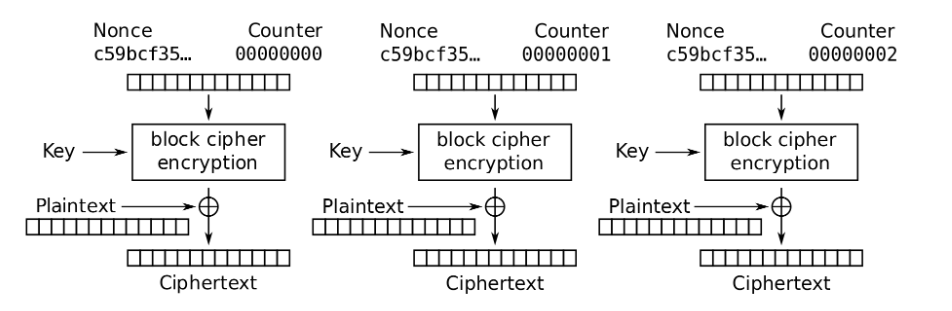
\includegraphics[width=1\linewidth]{latex-img/CTR_encryption.png}
        \caption{Counter (CTR) mode encryption}
        \label{ctr encryption}
    \end{figure}

    \item \textbf{Selection of Indices}: The algorithm iterates through the generated pseudorandom sequence, selecting the first \(m\) indices corresponding to vein pixels in the biometric template \(X\). This selection process involves a careful mechanism to ensure the uniqueness and proper ordering of indices.

    \item \textbf{Handling the Case \(m >\) (Number of 1's in Vein Image)}: In scenarios where the specified number of vein pixels \(m\) cannot be found due to the absence of sufficient vein pixels within the biometric template, the algorithm incorporates a built-in mechanism to address such situations. Before executing the prehash algorithm, it iterates through the image and verifies if the count of pixels equal to 1 is less than \(m\).

\end{itemize}

\begin{figure}[H]
    \centering
    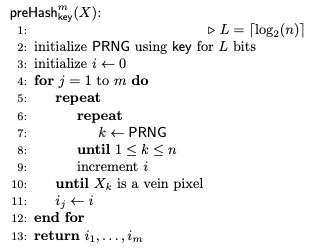
\includegraphics[width=0.5\linewidth]{latex-img/pseudocode_preHash.png}
    \caption{\textit{preHash} Algorithm}
    \label{preHash Algorithm}
\end{figure}

The algorithm, preHash, illustrated in Figure~\ref{preHash Algorithm} generates \(m\) smallest indices, denoted by \(i_j\), such that \(j\in{[1, m]} \) and \(1 <= i_1 < ... < i_m\), where each \(i_j\) correponds to an index such that \(X_{PRNG_{key}(i_j)} = 1\). It achieves this by rigorously verifying that the numbers produced by PRNG (PRNG[i]) stay within the specified bounds \(\text{PRNG}[i] \in (0, n] \text{ for } i \in [0, m]\).

\subsection{Assessing Similarity of Biometric Inputs After PreHash Application}

After the finger images are processed through the pipeline described in Pipeline~\ref{pipeline_simon} to extract their feature vectors, and the \textit{preHash} algorithm is applied, the outcome is a set of indices that fall within the inclusive range \(\text{PRNG}[i] \in (0, n] \text{ for } i \in [0, m]\), effectively mapping each selected feature to a unique index within the feature vector's length.

In the context of a simplified scenario where the hash length parameter (\(m\)) is set to \(1\), implying the generation of a single-index hash, and assuming a randomly chosen key for the \textit{preHash} algorithm, along with \(k\) representing a uniformly distributed random index, the probability that the \textit{preHash} operation yields the same index for two different inputs \(X\) and \(Y\) can be mathematically delineated as follows:

\begin{equation} \label{eq:preHash1}
    \begin{aligned}
        Pr[preHash_{key}^1(X) = preHash_{key}^1(Y)] &= \sum_{i > 0} Pr[preHash_{key}^1(X)]\\
        &= preHash_{key}^1(Y)\\
        &= \sum_{i > 0} Pr[X_k = Y_k = 0]^{i - 1} Pr[X_k = Y_k = 1]\\
        &= \frac{Pr[X_k = Y_k = 1]}{1 - Pr[X_k = Y_k = 0]}\\
        &= \frac{HW(X \land Y)}{HW(X) + HW(Y) - HW(X \land Y)}\\
        &= \frac{1}{\frac{1}{Score(X, Y)} - 1}
    \end{aligned}
\end{equation}

This equation encapsulates the likelihood of two images, \(X\) and \(Y\), having their singular hash index coincide, based on the presence of matching features identified by the algorithm. The final form of the equation relates the probability to the scoring function between \(X\) and \(Y\), inversely proportional to the score minus one.

It is noticed that there is a direct link with the Miura matching score that is of interest. The direct link between the \textit{preHash} algorithm's outcomes and the Miura matching score lies in their shared foundation of evaluating biometric similarities. Specifically, both methodologies utilize Hamming weight and bitwise operations to assess the overlap between biometric samples, such as finger vein patterns. The \textit{preHash} algorithm, through its probabilistic formula, quantifies the likelihood of matching indices based on feature presence, closely paralleling the Miura score's approach of comparing binary patterns to derive a similarity score. The above computation can also be expressed as follows:

\begin{equation} \label{eq:preHash2}
    \begin{aligned}
        Pr[preHash_{key}^1(\bar{X}) = preHash_{key}^1(\bar{Y})] &= \frac{Pr[\bar{X}_k = \bar{Y}_k = 1]}{1 - Pr[\bar{X}_k = \bar{Y}_k = 0]}\\
        &= \frac{\frac{Pr[X_k = 1] + Pr[Y_k = 1]}{2} - \frac{1}{2}Pr[\bar{X}_l \neq \bar{Y}_k]}{\frac{Pr[X_k = 1] + Pr[Y_k = 1]}{2} + \frac{1}{2}Pr[\bar{X}_l \neq \bar{Y}_k]}\\
    \end{aligned}
\end{equation}

The following approximations are made, inspired by equations p (\ref{eq:proba}) and $\delta$ (\ref{eq:delta}):

\begin{equation}
    E\left(\frac{\frac{Pr[X_k = 1] + Pr[Y_k = 1]}{2} - \frac{1}{2}Pr[\bar{X}_l \neq \bar{Y}_k]}{\frac{Pr[X_k = 1] + Pr[Y_k = 1]}{2} + \frac{1}{2}Pr[\bar{X}_l \neq \bar{Y}_k]}\right) \approx \frac{p - \frac{\delta}{2}}{p + \frac{\delta}{2}}
\end{equation}

The core of this approximation revolves around the expectation formula, which integrates probabilities of feature presence \(Pr[X_k=1]+Pr[Y_k=1]\) and the likelihood of discrepancies between \(X\) and \(Y\), \(Pr[\bar{X}_l \neq \bar{Y}_k]\). This formula essentially aims to quantify the similarity between two biometric samples by considering both the concurrence of features and the instances where they diverge.

Hence for (\(X\), \(Y\)) random,

\begin{equation}
    Pr[preHash_{key}^1(offset_X * X) = preHash_{key}^1(offset_Y * Y)] \leq \frac{p - \frac{\delta}{2}}{p + \frac{\delta}{2}}
\end{equation}

where equality is reached for the optimal offset translations. 

Depending on the distribution of (\(X\), \(Y\)), it is denoted

\begin{equation} \label{eq:mu}
    \mu = \frac{p - \frac{\delta}{2}}{p + \frac{\delta}{2}}
\end{equation}

The following figures are provided:

\begin{table}[H]
    \centering
    \renewcommand{\arraystretch}{1.25}\begin{tabular}{|c|c|c|}
        \hline
        $\mu_{same}$ & $\mu_{diff}$ & $\mu_{indep}$\\
        \hline
        $24\%$ & $8.3\%$ & $1.8\%$\\
        \hline
    \end{tabular}
\caption{Comparison of Distributions: $\delta_{same}$, $\delta_{diff}$, and $\delta_{indep}$}
\end{table}

Finally, it is observed that

\begin{equation}
    Pr[preHash_{key}^m(offset_X * X) = preHash_{key}^m(offset_Y * Y)] \leq \mu^m
\end{equation}

where equality is reached for the optimal offset translations.

%This includes determining the upper limits for the probabilities of similarity between different finger veins processed through the same fuzzy hashing parameters. 
\subsection{Experimental Derivation of the Probabilities \(\mu_{\text{same}}, \mu_{\text{diff}}, \mu_{\text{indep}}\)}

% Start this subsection by introducing the mathematical and theoretical concepts that underpin fuzzy hashing. Discuss the relevance of these concepts in the context of biometric data, focusing on how they enable the creation of reliable and secure hashing mechanisms for inherently noisy data.

%     Key Concepts to Cover:
%         Definition and significance of fuzzy hashing
%         Mathematical principles governing the construction of fuzzy hashes
%         Overview of the biometric setting, including the importance of parameters such as pixel dimensions, vein extraction, and the role of random permutations in hashing

% Subsection 2: Experimental Approach

% In the second subsection, outline the methodology of your experiments designed to test the theoretical underpinnings discussed earlier. Describe the setup, the specific objectives of each experiment, and how these experiments are structured to validate the theoretical models of fuzzy hashing.

%     Key Components to Include:
%         Description of the experimental setup and the data used
%         Explanation of how the experiments are designed to reflect the theoretical aspects of fuzzy hashing
%         Details on the implementation of preHash and postHash functions, and the criteria for their evaluation

% Subsection 3: Verifying Theoretical Predictions

% The final subsection is dedicated to comparing the outcomes of your experiments with the theoretical expectations. This involves analyzing the results, discussing any deviations or confirmations, and what these mean for the validity and reliability of fuzzy hashing in biometric data security.

%     Important Aspects to Discuss:
%         Analysis of experimental results against theoretical predictions
%         Discussion on the accuracy of the fuzzy hashing process, including the matching scores and error rates
%         Implications of the findings for biometric data security and future research directions

% Conclusion of Section 1

% Conclude with a summary of the insights gained from bridging theoretical concepts with empirical evidence. Highlight the importance of this integration for advancing the field of biometric security through fuzzy hashing. Reflect on the potential for future developments and applications stemming from your findings. --> Avons nous vraiment besoin de ça dans cette partie?
\newpage
\section{Introduction}

\subsection{Background}
Authentication is the process of confirming the validity of a claimed identity seeking access to a system or resource. Over decades, authentication mechanisms have evolved from basic password systems in the 1960s to advanced methods such as multifactor authentication by the late 2010s, driven by a persistent commitment to combat evolving security risks while enhancing user convenience\cite{ref1}. Various methods such as password-based authentication, certificate-based authentication, one-time passwords, multifactor authentication, and biometric authentication are employed\cite{ref2}.

Biometric authentication, which involves analyzing unique physical characteristics, is often considered more secure than traditional authentication methods due to the difficulty in duplicating biometric traits. This encompasses technologies such as facial recognition, fingerprint recognition, eye recognition, and voice recognition\cite{ref3}.
However, despite the enhanced security of biometric authentication, it is not immune to exploitation. For instance, fingerprints left on surfaces can be copied, or hackers may obtain images of individuals online to deceive authentication systems.
Choosing the right authentication mechanism requires careful consideration of various factors including the necessary security level, ease of use for users, cost implications for setup and ongoing upkeep, as well as the unique risks and vulnerabilities pertinent to the system or data in question. Typically, the requisite level of security steers the selection process; for example, platforms managing sensitive personal information might mandate the use of robust authentication methods, such as biometric verification. The inherent challenge in deploying such secure systems lies in achieving a delicate equilibrium between high security measures and user convenience. The goal is to create an authentication process that is both seamless and efficient, ensuring that access is granted swiftly and accurately to the rightful user without necessitating multiple attempts, thus maintaining a user-friendly experience while upholding the highest security standards.

While advanced biometric systems typically rely on externally visible physical attributes, finger-vein authentication focuses on internal anatomical features, adding a unique layer of security, as they are less prone to replication or theft compared to external characteristics. Nevertheless, it is important to note that finger-vein authentication does not completely eliminate challenges. Despite its emphasis on internal features, attackers can exploit inherent structures in finger veins, such as common patterns among individuals and predictability in acquired data, which poses risks to the authentication process.\\

In light of these considerations, this project is dedicated to authentication using finger-vein features.
This involves utilizing a specialized scanner equipped with two infrared cameras to capture finger veins from different angles.
The registration process involves capturing an image, termed the model image, while the authentication process involves capturing another image, known as the probe image. These images undergo processing through a pipeline designed to extract and align the finger-vein patterns.
The pipeline outputs a feature vector, which is essentially a bitstring, where 0's represent where there are no finger veins, and 1's show where veins are present.
Following this process, the system evaluates whether the feature vector extracted from the probe image sufficiently matches the feature vector of the model image associated with the individual attempting authentication.

\subsection{Extraction Pipeline}\label{sec:extraction-pipeline}

This project extends the work on optimizing a finger-vein recognition pipeline that has demonstrated the lowest \hyperref[def:EER]{Equal Error Rate (EER)} by incorporating a novel hashing step to process the output of the pipeline. The purpose of integrating \hyperref[def:Hash_Function]{Hash Functions} within this context is multifold, but before delving into hash functions, which are central to our project, it's essential to outline the foundation upon which we have built our advancements. This initial context will provide a clearer understanding of the starting point from which our developments began.\\

Simon Sommerhalder and Burcu Yildiz have both made significant contributions to the system. Simon introduced an innovative approach to the alignment of freshly captured images (probe images) with those stored in the system (model images), ensuring the hashing process (following the alignment of the finger) is based on the unique finger-vein pattern rather than how the finger is positioned on the scanner.

Simon has developped a pipeline (see Figure~\ref{pipeline_simon}) to align finger-vein images, enhancing security by eliminating the need to compare the model and probe images side by side. He organized the pipeline into six clear steps:

\begin{enumerate}
    \item \textbf{Masking}: The first step of the pipeline isolates the finger area in the image. This involves creating a mask that outlines the finger, ensuring that subsequent processing focuses solely on the relevant part of the image.

    \item \textbf{Prealignment}: This step involves adjusting the position and orientation of the finger within the image before extracting vein patterns. It's aimed at roughly aligning the image based on the finger's outline, helping to standardize the position of the finger across different scans.

    \item \textbf{Histogram equalization}: To ensure the images have consistent lighting and contrast, this step adjusts the brightness levels. This makes the vein patterns more distinct and comparable across different images.

    \item \textbf{Feature extraction}: Here, the actual vein patterns are identified and extracted from the image. The process converts the visual image into a digital format that represents the presence or absence of veins at specific locations.

    \item \textbf{Postalignment}: After extracting the vein patterns, this step fine-tunes the alignment of the image. It's based on the vein patterns themselves, ensuring that the comparison between model and probe images is as accurate as possible.

    \item \textbf{Distance Calculation}: The final step involves comparing the feature vector of the probe image with that of the model image. This is done using a specific metric to quantify the similarity between the two, ultimately determining if they match closely enough for authentication to succeed.
\end{enumerate} 

\begin{figure}[!h]
    \centering
    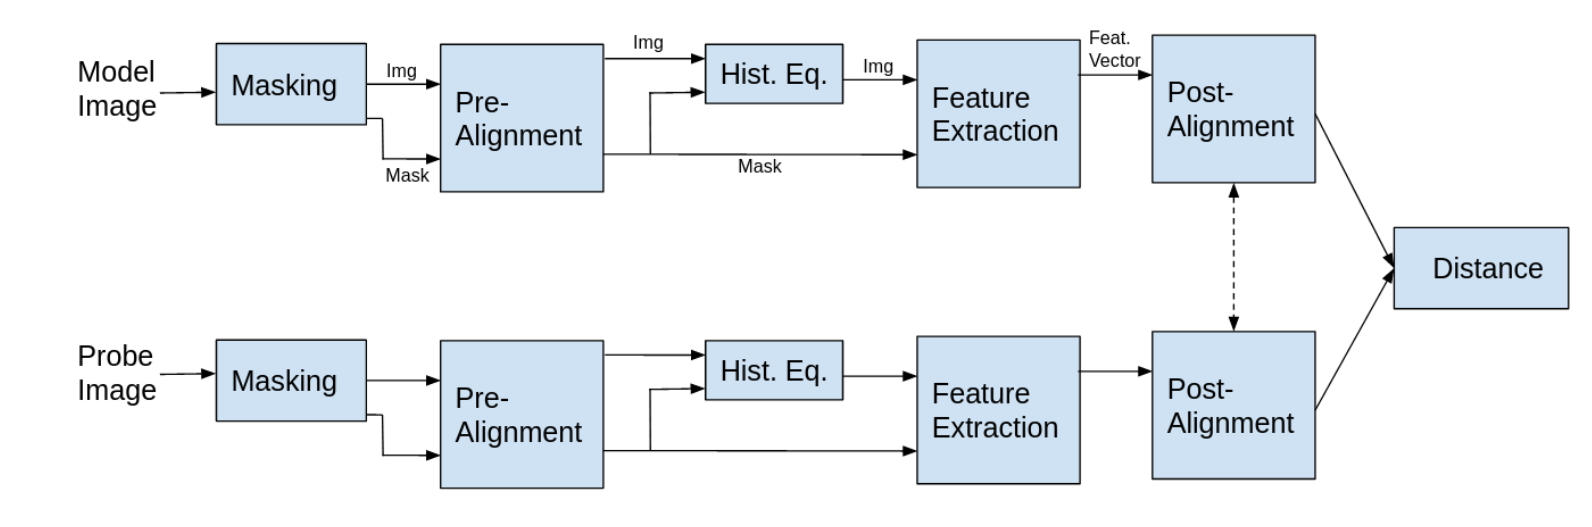
\includegraphics[width=1\linewidth]{latex-img/pipeline_simon.png}
    \caption{Simon's Extraction Pipeline. Compares a single probe image to a model image}
    \label{pipeline_simon}
\end{figure}

Burcu's work on the finger vein authentication project built upon Simon's foundational pipeline, focusing on refining image processing for vein extraction and evaluating different distance calculation methods for authentication. She optimized preprocessing steps, investigated masking and prealignment issues, and tackled reference selection to enhance matching accuracy. A significant part of her contributions involved exploring fuzzy extractors \hyperref[def:Fuzzy_Extractors]{Fuzzy Extractors} to bolster security, conducting a thorough analysis of the dataset to identify and address challenges, and proposing solutions to improve the system's reliability and efficiency.\\

Simon and Burcu explored a variety of function combinations at different stages of the authentication pipeline, aiming to pinpoint the configuration that yields the most favorable outcomes. They utilized the Equal Error Rate (EER) as a benchmark to measure the pipeline's efficacy, focusing on achieving a balance between security and accessibility. This metric, representing the point where the rate of false acceptances (impostor incorrectly granted access) matches the rate of false rejections (legitimate user incorrectly denied), serves as an indicator of the system's reliability and accuracy. The configuration that demonstrated superior performance, leading to the lowest EER and thereby optimizing the process of analyzing and processing images, is showcased in the subsequent figure.

\begin{table}[H]
    \centering
    \caption{EER values for the best pipeline: Edge masking, translation pre-alignment, no pre-processing, no post-
    processing, Miura matching as the post-alignment}
    \begin{tabular}{lc}
    \toprule
    Camera & EER \\
    \midrule
    Camera 1 & 0.041 \\
    Camera 2 & 0.029 \\
    Sum of cameras & 0.030 \\
    \bottomrule
    \end{tabular}
    \label{tab:eervalues_best}
\end{table}

\subsection{Project Overview}

In the progression of our project, building upon the work of Simon and Burcu, we aim to address the inherent variability in biometric data, particularly with finger vein patterns, by considering hash functions. The final objective of the system is to add a hashing step at the end of our established pipeline, prior to the post-alignment phase. The integration of this step serves to enhance security and overall functionality by allowing us to store a hash of each biometric image X in our database, instead of the raw biometric data. Upon receiving a new image Y, we compute hashes for all potential translations of Y, comparing these with the hash of X. Unfortunately, this process is computationally expensive because it requires computing the hash for every possible translation of the image. The purpose of employing a hashing process in this system is multifold:

\begin{itemize}
    \item \textbf{Security}: Hash values can be stored instead of raw biometric data. In the event of a database breach, attackers would find it significantly more challenging to reconstruct the original biometric information from the hashed values due to the one-way nature of hash functions.

    \item \textbf{Consistency}: By focusing on the unique patterns of the biometric trait (like finger-vein patterns) and standardizing how this data is processed and hashed, the system aims to produce consistent hash values for the same individual across different scanning sessions. This is crucial for reliable authentication, ensuring that minor variations in finger placement do not affect the system's ability to recognize the user.

    \item \textbf{Performance}: Hashing biometric data into a compact, fixed-size format facilitates quicker comparison and verification processes. It's more efficient to compare hash values than to perform complex pattern recognition operations on raw biometric images.
\end{itemize}

Traditional hash functions, while pivotal in various data security contexts, generate a unique output for each unique input. This one-to-one mapping means even minor variations in the input — common in biometric data due to natural changes in biological traits or differences in scanning conditions — result in completely different hashes. This sensitivity to input variability poses a challenge in biometric authentication systems, where the goal is to accurately recognize and authenticate an individual despite these natural variations.

Fuzzy hashing stands as a sophisticated solution to this challenge. Unlike traditional hash functions, fuzzy hashing is designed to produce consistent cryptographic keys for inputs that are similar, but not identical. This is particularly advantageous in biometric authentication systems, where it's essential to recognize the same biometric trait across different instances, despite slight variations. The "fuzziness" of this approach allows the system to map these similar inputs to the same or closely related hash values, thereby ensuring that legitimate users are not incorrectly denied access due to minor discrepancies in their biometric data.
Furthermore, the application of fuzzy hashing in our pipeline is instrumental in protecting user privacy. Since the hashed values, rather than raw biometric data, are stored and used for authentication, users' biometric information is safeguarded against potential breaches. Even if hashed values were accessed without authorization, the complexity of fuzzy hashing algorithms makes it extremely challenging to reverse-engineer the original biometric data.\\

The process of our fuzzy hashing algorithm, that we will detail in Section~\ref{sec:Fuzzy Hashing}  begins with a biometric capture, a finger image, which goes through the already developped pipeline~\ref{pipeline_simon} to extract a bitstring. This bitstring undergoes a pre-hashing process, where a subset of significant bits (denoted as vein pixels) is selected based on a permutation keyed by a secure key, resulting in a tuple that significantly reduces the data's dimensionality while preserving its distinguishing features.

Upon generating the fuzzy hash, the next step involves further compressing this hash to prepare it for storage. This compression is achieved through a function, postHash, which maps the tuple to a bitstring of a defined length. The output, essentially a compressed fuzzy hash, exhibits nearly uniform distribution when both the input data and the key are random, enhancing security and storage efficiency.

To further bolster the security of the stored biometric data, this system incorporates \hyperref[def:Fuzzy_Extractors]{Fuzzy Extractors}. The fuzzy extractor framework ensures that even if the stored data is compromised, reconstructing the original biometric data or compromising individual privacy remains computationally infeasible. This is accomplished by generating a secure, random key from the biometric input using a generation process (Gen) and allowing for the reliable reproduction of this key from an approximation of the original input using a reproduction process (Rep), without directly storing the biometric data itself.

In essence, we aim to store the output of the fuzzy extractor, which includes the reproducible cryptographic key and the helper data, instead of the raw biometric data or its direct hash. This method ensures that the stored biometric data is not only compact and efficiently stored but also securely obfuscated, requiring the correct biometric input for any form of decryption or matching to occur.



\section{Fuzzy Hashing}
\label{sec:Fuzzy Hashing}
Fuzzy hashing, as opposed to traditional hashing, produces consistent cryptographic keys for similar but not identical inputs, enabling recognition of the same biometric trait across different instances despite slight variations. This approach ensures legitimate users are not incorrectly denied access due to minor discrepancies and protects user privacy by storing and using hashed values instead of raw biometric data, making it difficult to reverse-engineer the original data even if unauthorized access occurs. 
This section will discuss how we implemented the fuzzy hashing algorithm, its corresponding mathematical aspects and some experiments.

\subsection{PreHashing Algorithm}

The \textit{PreHash} algorithm is the first step in the fuzzy hashing process, designed to manipulate biometric templates extracted from finger vein patterns. It operates on a bitstring \(X\), representing the presence (1) or absence (0) of vein pixels across \(n\) pixels, where \(n=96'500\).

Algorithm Inputs and Outputs:
\begin{enumerate}
    \item \textbf{Inputs}: The algorithm takes three main inputs:
    \begin{itemize}
        \item \textbf{A parameter m}: the number of indices to find
        \item \textbf{A bitstring X}: the feature-extracted vein patterns of a biometric capture
        \item \textbf{A key}: used to initialize a Pseudorandom Number Generator (PRNG)
    \end{itemize}
    \item \textbf{Output}: The algorithm outputs a tuple \((i_1,...,i_m)\) consisting of the \(m\) smallest indices \(i_j\)​ such that \(1 \leq i_1<...<i_m\)​ and the pixel at \(PRNGkey(i_j)\) in \(X\) is identified as a vein pixel. 
\end{enumerate}

Detailed Process of \textit{PreHash}:
\begin{itemize}
    \item \textbf{Initiallization}: Utilizing the provided key, the algorithm initializes a PRNG. This PRNG is based on the \hyperref[def:AES CTR mode]{Advanced Encryption Standard (AES) in Counter (CTR) mode}, ensuring the generation of uniform and independent pseudorandom sequences.

    \item \textbf{Nonce Generation}: A nonce in CTR mode encryption is initialized to zero to maintain simplicity and security. We opted against using a keyed hash function to generate the nonce, as it would tie the nonce to the secret key. Such a dependency would mean that both the nonce and the Pseudo-Random Number Generator (PRNG) would rely on the same key, creating a security risk by concentrating security on a single element. To avoid this, we keep the generation of the nonce separate from the key.

    \item \textbf{Pseudorandom Sequence Generation}: Upon receiving the parameters—key, nonce, and counter—the PRNG operates in CTR mode to generate a 128-bit pseudo-random number. As depicted in Figure~\ref{ctr encryption}, this process involves encrypting the nonce combined with the counter using the key. The output from this block cipher encryption phase is then XORed with a vector consisting of zero bits. Since we require 17 bits for our application, the block cipher's output is XORed with a bitstring of 3 bytes to achieve the necessary length. To ensure the output meets the project's specific requirements, it is then masked to retain only the top 17 bits. This adjustment is essential as it aims to ensure that pseudo-random numbers are generated within a suitable range form image size, specifically \(96'500\) pixels, which requires \(17\) bits for representation\footnote{\(\lceil \log_2(96'500) \rceil = 17\)}. The predictability of this sequence is entirely dictated by the chosen key. In essence, employing the same key will consistently yield an identical nonce and hence an identical sequence of numbers.

    \begin{figure}[!h]
        \centering
        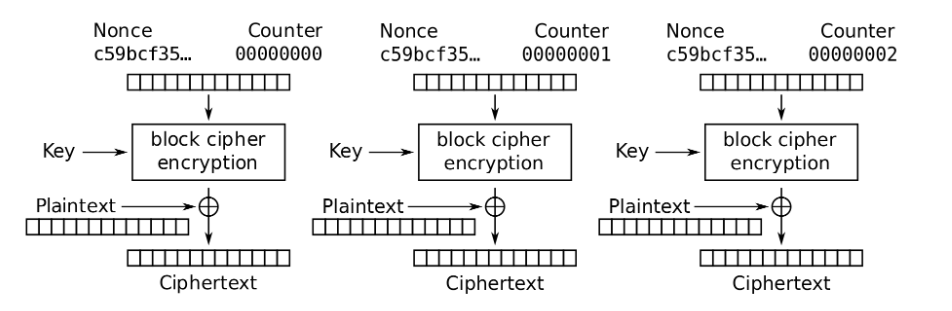
\includegraphics[width=1\linewidth]{latex-img/CTR_encryption.png}
        \caption{Counter (CTR) mode encryption}
        \label{ctr encryption}
    \end{figure}

    \item \textbf{Selection of Indices}: The algorithm iterates through the generated pseudorandom sequence, selecting the first \(m\) indices corresponding to vein pixels in the biometric template \(X\). This selection process involves a careful mechanism to ensure the uniqueness and proper ordering of indices.

    \item \textbf{Handling the Case \(m >\) (Number of 1's in Vein Image)}: In scenarios where the specified number of vein pixels \(m\) cannot be found due to the absence of sufficient vein pixels within the biometric template, the algorithm incorporates a built-in mechanism to address such situations. Before executing the prehash algorithm, it iterates through the image and verifies if the count of pixels equal to 1 is less than \(m\).

\end{itemize}

\begin{figure}[H]
    \centering
    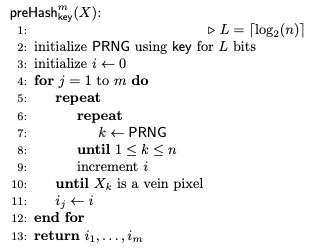
\includegraphics[width=0.5\linewidth]{latex-img/pseudocode_preHash.png}
    \caption{\textit{preHash} Algorithm}
    \label{preHash Algorithm}
\end{figure}

The algorithm, preHash, illustrated in Figure~\ref{preHash Algorithm} generates \(m\) smallest indices, denoted by \(i_j\), such that \(j\in{[1, m]} \) and \(1 <= i_1 < ... < i_m\), where each \(i_j\) correponds to an index such that \(X_{PRNG_{key}(i_j)} = 1\). It achieves this by rigorously verifying that the numbers produced by PRNG (PRNG[i]) stay within the specified bounds \(\text{PRNG}[i] \in (0, n] \text{ for } i \in [0, m]\).

\subsection{Assessing Similarity of Biometric Inputs After PreHash Application}

After the finger images are processed through the pipeline described in Pipeline~\ref{pipeline_simon} to extract their feature vectors, and the \textit{preHash} algorithm is applied, the outcome is a set of indices that fall within the inclusive range \(\text{PRNG}[i] \in (0, n] \text{ for } i \in [0, m]\), effectively mapping each selected feature to a unique index within the feature vector's length.

In the context of a simplified scenario where the hash length parameter (\(m\)) is set to \(1\), implying the generation of a single-index hash, and assuming a randomly chosen key for the \textit{preHash} algorithm, along with \(k\) representing a uniformly distributed random index, the probability that the \textit{preHash} operation yields the same index for two different inputs \(X\) and \(Y\) can be mathematically delineated as follows:

\begin{equation} \label{eq:preHash1}
    \begin{aligned}
        Pr[preHash_{key}^1(X) = preHash_{key}^1(Y)] &= \sum_{i > 0} Pr[preHash_{key}^1(X)]\\
        &= preHash_{key}^1(Y)\\
        &= \sum_{i > 0} Pr[X_k = Y_k = 0]^{i - 1} Pr[X_k = Y_k = 1]\\
        &= \frac{Pr[X_k = Y_k = 1]}{1 - Pr[X_k = Y_k = 0]}\\
        &= \frac{HW(X \land Y)}{HW(X) + HW(Y) - HW(X \land Y)}\\
        &= \frac{1}{\frac{1}{Score(X, Y)} - 1}
    \end{aligned}
\end{equation}

This equation encapsulates the likelihood of two images, \(X\) and \(Y\), having their singular hash index coincide, based on the presence of matching features identified by the algorithm. The final form of the equation relates the probability to the scoring function between \(X\) and \(Y\), inversely proportional to the score minus one.

It is noticed that there is a direct link with the Miura matching score that is of interest. The direct link between the \textit{preHash} algorithm's outcomes and the Miura matching score lies in their shared foundation of evaluating biometric similarities. Specifically, both methodologies utilize Hamming weight and bitwise operations to assess the overlap between biometric samples, such as finger vein patterns. The \textit{preHash} algorithm, through its probabilistic formula, quantifies the likelihood of matching indices based on feature presence, closely paralleling the Miura score's approach of comparing binary patterns to derive a similarity score. The above computation can also be expressed as follows:

\begin{equation} \label{eq:preHash2}
    \begin{aligned}
        Pr[preHash_{key}^1(\bar{X}) = preHash_{key}^1(\bar{Y})] &= \frac{Pr[\bar{X}_k = \bar{Y}_k = 1]}{1 - Pr[\bar{X}_k = \bar{Y}_k = 0]}\\
        &= \frac{\frac{Pr[X_k = 1] + Pr[Y_k = 1]}{2} - \frac{1}{2}Pr[\bar{X}_l \neq \bar{Y}_k]}{\frac{Pr[X_k = 1] + Pr[Y_k = 1]}{2} + \frac{1}{2}Pr[\bar{X}_l \neq \bar{Y}_k]}\\
    \end{aligned}
\end{equation}

The following approximations are made, inspired by equations p (\ref{eq:proba}) and $\delta$ (\ref{eq:delta}):

\begin{equation}
    E\left(\frac{\frac{Pr[X_k = 1] + Pr[Y_k = 1]}{2} - \frac{1}{2}Pr[\bar{X}_l \neq \bar{Y}_k]}{\frac{Pr[X_k = 1] + Pr[Y_k = 1]}{2} + \frac{1}{2}Pr[\bar{X}_l \neq \bar{Y}_k]}\right) \approx \frac{p - \frac{\delta}{2}}{p + \frac{\delta}{2}}
\end{equation}

The core of this approximation revolves around the expectation formula, which integrates probabilities of feature presence \(Pr[X_k=1]+Pr[Y_k=1]\) and the likelihood of discrepancies between \(X\) and \(Y\), \(Pr[\bar{X}_l \neq \bar{Y}_k]\). This formula essentially aims to quantify the similarity between two biometric samples by considering both the concurrence of features and the instances where they diverge.

Hence for (\(X\), \(Y\)) random,

\begin{equation}
    Pr[preHash_{key}^1(offset_X * X) = preHash_{key}^1(offset_Y * Y)] \leq \frac{p - \frac{\delta}{2}}{p + \frac{\delta}{2}}
\end{equation}

where equality is reached for the optimal offset translations. 

Depending on the distribution of (\(X\), \(Y\)), it is denoted

\begin{equation} \label{eq:mu}
    \mu = \frac{p - \frac{\delta}{2}}{p + \frac{\delta}{2}}
\end{equation}

The following figures are provided:

\begin{table}[H]
    \centering
    \renewcommand{\arraystretch}{1.25}\begin{tabular}{|c|c|c|}
        \hline
        $\mu_{same}$ & $\mu_{diff}$ & $\mu_{indep}$\\
        \hline
        $24\%$ & $8.3\%$ & $1.8\%$\\
        \hline
    \end{tabular}
\caption{Comparison of Distributions: $\delta_{same}$, $\delta_{diff}$, and $\delta_{indep}$}
\end{table}

Finally, it is observed that

\begin{equation}
    Pr[preHash_{key}^m(offset_X * X) = preHash_{key}^m(offset_Y * Y)] \leq \mu^m
\end{equation}

where equality is reached for the optimal offset translations.

%This includes determining the upper limits for the probabilities of similarity between different finger veins processed through the same fuzzy hashing parameters. 
\subsection{Experimental Derivation of the Probabilities \(\mu_{\text{same}}, \mu_{\text{diff}}, \mu_{\text{indep}}\)}

% Start this subsection by introducing the mathematical and theoretical concepts that underpin fuzzy hashing. Discuss the relevance of these concepts in the context of biometric data, focusing on how they enable the creation of reliable and secure hashing mechanisms for inherently noisy data.

%     Key Concepts to Cover:
%         Definition and significance of fuzzy hashing
%         Mathematical principles governing the construction of fuzzy hashes
%         Overview of the biometric setting, including the importance of parameters such as pixel dimensions, vein extraction, and the role of random permutations in hashing

% Subsection 2: Experimental Approach

% In the second subsection, outline the methodology of your experiments designed to test the theoretical underpinnings discussed earlier. Describe the setup, the specific objectives of each experiment, and how these experiments are structured to validate the theoretical models of fuzzy hashing.

%     Key Components to Include:
%         Description of the experimental setup and the data used
%         Explanation of how the experiments are designed to reflect the theoretical aspects of fuzzy hashing
%         Details on the implementation of preHash and postHash functions, and the criteria for their evaluation

% Subsection 3: Verifying Theoretical Predictions

% The final subsection is dedicated to comparing the outcomes of your experiments with the theoretical expectations. This involves analyzing the results, discussing any deviations or confirmations, and what these mean for the validity and reliability of fuzzy hashing in biometric data security.

%     Important Aspects to Discuss:
%         Analysis of experimental results against theoretical predictions
%         Discussion on the accuracy of the fuzzy hashing process, including the matching scores and error rates
%         Implications of the findings for biometric data security and future research directions

% Conclusion of Section 1

% Conclude with a summary of the insights gained from bridging theoretical concepts with empirical evidence. Highlight the importance of this integration for advancing the field of biometric security through fuzzy hashing. Reflect on the potential for future developments and applications stemming from your findings. --> Avons nous vraiment besoin de ça dans cette partie?

\section{Compressed Fuzzy Hashing}
\label{sec:Compressed Fuzzy Hashing}

Compressed fuzzy hashing generates concise hashes of data, capturing key features while allowing for slight variations - a concept referred to as "fuzziness". Unlike conventional cryptographic hashing, which generates fixed-length outputs and is highly sensitive to even minimal changes in input, compressed fuzzy hashing maintains a robust link to the original content despite alterations.
This section delves into the mechanics of the compressed fuzzy hashing algorithm, called the postHash procedure. We will explore the mathematical concepts that enable its effectiveness and discuss experimental results that demonstrate its capabilities and performance on our dataset.

\subsection{PostHashing Algorithm}

The postHash algorithm, constituting the second and final step in the fuzzy hashing process, generates compact hashes based on the indices derived from the preHash algorithm (see Section \ref{sec:Fuzzy Hashing}). This algorithm is designed to transform a tuple of indices into a concise hash format, \(h_1 || \ldots || h_m\), where each \(h_i\), for \(i \in [1, m]\), is an integer within the range \([0, \ldots, D-1]\).The parameter \(D\), defined as \(2^d\), denotes the total number of possible values each \(h_i\) can assume, with \(d\) representing the bit depth used per index. 

Algorithm Inputs and Outputs:
\begin{enumerate}
    \item \textbf{Inputs}: As illustrated in Figure~\ref{postHash Algorithm}, the algorithm takes as input:
    \begin{itemize}
        \item \textbf{A tuple of indices}: \((i_1, \ldots, i_m)\), which is the output of the preHash algorithm
    \end{itemize}
    \item \textbf{Output}: Converted indices, forming a compact hash \(h_1|| \ldots || h_m\), where \(h_i\) \(i \in [1, m]\), is an integer in \([0, \ldots, D-1]\)
\end{enumerate}

Detailed process of postHash, for the case when $d < 4$:
\begin{enumerate}
    \item \textbf{Subroutine}: For each index provided by the preHash, subroutine \(T\) checks if the index is within the acceptable range. If an index is out of range, \(T\) returns 0, otherwise, it proceeds with a table lookup. The subroutine maps each valid index \(i\) to an integer nearly uniformly distributed between \([0, D-1]\), ensuring that all potential hash values are equally probable. This mapping is important for the security and effectiveness of the fuzzy hashing system.
    
    The subroutine function, \(T\), works as follows:
    \begin{itemize}
        \item \textbf{Inputs}: 
        \begin{itemize}
            \item \textbf{Shifted Index}: Each index from the preHash output tuple \((i_1, \ldots, i_m)\) is adjusted before conversion into a hash component. Specifically, the index \(i\) is shifted by subtracting a previously determined index \(i'\), resulting in a transformed index \(i - i'\). This shifting process normalizes the indices, maintaining a consistent relative positioning within the dataset, which helps in achieving a more uniform distribution of hash values across the range \([0, D-1]\).
            \item \textbf{d}: Represents the bit length used for each hash index \(h_i\). This value determines \(D = 2^d\), the total number of distinct values each \(h_i\) can take, effectively setting the hash resolution.
        \end{itemize}
        \item \textbf{Output}: \(h_i\), the mapped integer
    \end{itemize}
\end{enumerate}

For the case when $d = 4$, a different subroutine called \textit{scambled\_T} is used. This subroutine corresponds to a partition problem, which is detailed at the end of Section~\ref{sec:Experimental_derivation_q}. Although the mapping of integers differs in this subroutine, it similarly takes an index from the preHash tuple as input and maps it to an integer, just as in the process for $d < 4$.

\vspace{20pt}

\begin{algorithm}
    \begin{algorithmic}[1]
    \caption{postHash Algorithm}
    \label{postHash Algorithm}
    \Function{(postHash $\circ$ preHash$_\text{key}^m$)}{$X$}
    \State $\text{hash} = []$
    \State $i' \gets 0$
    \For{$i \in \text{indices}$}
        \State $h_i \gets \text{Subroutine}(i - i', d)$
        \State $\text{hash.append}(h_i)$
        \State $i' \gets i$
    \EndFor 
    \State \Return{$h_1, \ldots, h_m$}
    \EndFunction
    \end{algorithmic}
    \end{algorithm}
    
    \begin{algorithm}
    \begin{algorithmic}[1]
    \caption{\textit{Subroutine} Algorithm}
    \label{Subroutine Algorithm}
    \Function{\text{Subroutine}}{$i$, $d$}
    \State $p = 0.03514$
    \State $h_i = \lfloor 2^d (1-p)^{i} \rfloor$
    \State \Return{$h_i$}
    \EndFunction
    \end{algorithmic}
    \end{algorithm}

\subsection{Assessing Similarity of Biometric Inputs After PostHash Application}
\label{sec:q}

After processing finger images through the pipeline referenced in Pipeline~\ref{pipeline_simon} to extract their feature vectors, the resulting data undergo the preHash and subsequently, the postHash algorithms. The final output from postHash consists of a set of integers \( h_i \), each bounded within the inclusive range \([0, D-1]\). This process effectively assigns each feature vector index to an integer within this range.

In our methodology, we model these integers \( h_i \) as following a geometric distribution. This assumption is based on the output relationship established by \( Hash_{key}^m(X) = postHash(preHash_{key}^m(X)) \). We assume the same conditions as discussed in Section~\ref{sec:Fuzzy Hashing}: the key is randomly chosen, and \(k\) represents a uniformly distributed random index. Consequently, the probability of the Hash operation yielding the same index for two different inputs \(X\) and \(Y\) can be mathematically characterized as follows:

\[Pr[Hash_{key}^m(d_X) = Hash_{key}^m(d_Y)] \leq \mu^m(1 - \frac{1}{D}) + \frac{1}{D}\]

where equality is reached for the optimal offset translations.

The overall probability \( q \) of a matching hash index under random inputs \( X \) and \( Y \), reflecting their distribution, is denoted by:

\begin{equation}
    q = \mu^m\left(1 - \frac{1}{D}\right) + \frac{1}{D}
    \label{eq:q_formula}
\end{equation}
    

Based on the range of possible values for \(d\), we have computed several specific instances of \(q\) (theoretical values given by the above equation):
\begin{table}[H]
    \centering
    \renewcommand{\arraystretch}{1.25}\begin{tabular}{|c|c|c|c|}
        \hline
        & $q_{same}$ & $q_{diff}$ & $q_{indep}$\\
        \hline
        \(m = 1\) \(d = 1\) & $61.03\%$ & $54.12\%$ & $50.73\%$\\
        \(m = 1\) \(d = 2\) & $41.54\%$ & $31.19\%\%$ & $26.09\%$\\
        \(m = 1\) \(d = 3\) & $31.79\%$ & $19.72\%$ & $13.77\%$\\
        \(m = 1\) \(d = 4\) & $26.92\%$ & $13.98\%$ & $7.61\%$\\
        \hline
    \end{tabular}
\caption{Comparison of Distributions: $q_{same}$, $q_{diff}$, and $q_{indep}$}
\label{tab:theoretical_q}
\end{table}

\subsection{Experimental Derivation of the probabilities $q_{same}^{obs}$, $q_{diff}^{obs}$, and $q_{indep}^{obs}$ for different \(m\), \(d\) parameter combinations} \label{sec:Experimental_derivation_q}

In the subsequent section, we explore enhancements to data compression techniques within our fuzzy hashing framework, emphasizing the use of various \(m\) and \(d\) parameter combinations. We initiate our analysis by conducting experiments to determine \(q_{same}^{obs}\), \(q_{diff}^{obs}\), and \(q_{indep}^{obs}\).

Building on the foundational calculations for \(q_{\text{indep}}\), which we derived using Formula ~\ref{eq:q_formula} with \( \mu^{obs}_{\text{indep}} \) previously identified in Section \ref{sec:Fuzzy Hashing}, our exploration extended to \(q^{obs}_{\text{same}}\) and \(q^{obs}_\text{diff}\). To evaluate these parameters, we initiated a series of experiments. Integral to this implementation and the following ones, is the creation of the lookup table, to convert indices to their compressed counterparts. The generation of this table and all subsequent ones, is governed by a geometrically-derived formula that accurately encapsulates the transformation of index values. The specific formula is presented as:

\begin{equation}
    \text{postHash}(i) = \left\lfloor 2^d \left(1 - p\right)^i \right\rfloor
    \label{eq:GeomFormula}
\end{equation}
    
 
Leveraging the above formula, we have developed lookup tables that convert a single index (\(m = 1\)) into various bit representations (\(d=1\), \(d=2\), \(d=3\), and \(d=4\)). Each entry in these tables represents an integer, denoted by \(i\), and includes a corresponding hash output and the probability of that output occurring.

Binary Hash Output Distribution Table (\(d=1\))
{\renewcommand{\arraystretch}{1.25}
\[
\text{postHash}(i) = \left\{
    \begin{array}{lll}
        \text{1}  & \text{if } 1 \leq i \leq 19 & (\text{Pr} = 49.32\%)
        \\
        \text{0}  & \text{if } 20 \leq i & (\text{Pr} = 50.68\%)
        \\
    \end{array}
\right.    
\]}


Quaternary Hash Output Distribution Table (\(d=2\)):
{\renewcommand{\arraystretch}{1.25}
\[
\text{PostHash}(i) = \left\{
    \begin{array}{lll}
        \text{3}  & \text{if } 1 \leq i \leq 8 & (\text{Pr} = 24.89\%)
        \\
        \text{2}  & \text{if } 9 \leq i \leq 19 & (\text{Pr} = 24.43\%)
        \\
        \text{1}  & \text{if } 20 \leq i \leq 38 & (\text{Pr} = 25\%)
        \\
        \text{0}  & \text{if } 39 \leq i & (\text{Pr} = 25.68\%)
        \\
    \end{array}
\right.    
\]}

Octal Hash Output Distribution Table (\(d=3\)):
{\renewcommand{\arraystretch}{1.25}
\[
\text{postHash}(i) = \left\{
    \begin{array}{lll}
        \text{7}  & \text{if } 1 \leq i \leq 3 & (\text{Pr} = 10.18\%)
        \\
        \text{6}  & \text{if } 4 \leq i \leq 8 & (\text{Pr} = 14.71\%)
        \\
        \text{5}  & \text{if } 9 \leq i \leq 13 & (\text{Pr} = 12.3\%)
        \\
        \text{4}  & \text{if } 14 \leq i \leq 19 & (\text{Pr} = 12.13\%)
        \\
        \text{3}  & \text{if } 20 \leq i \leq 27 & (\text{Pr} = 12.61\%)
        \\
        \text{2}  & \text{if } 28 \leq i \leq 38 & (\text{Pr} = 12.38\%)
        \\
        \text{1}  & \text{if } 39 \leq i \leq 58 & (\text{Pr} = 13.12\%)
        \\
        \text{0}  & \text{if } 59 \leq i & (\text{Pr} = 12.59\%)
        \\
    \end{array}
\right.    
\]}


Hexadecimal Hash Output Distribution Table \(d=4\)
{
\renewcommand{\arraystretch}{1.25}
\[
\text{postHash}(i) = \left\{
\begin{array}{lll}
    \text{15} & \text{if } i = 1 & (\text{Pr} = 3.51\%), \\
    \text{14} & \text{if } 2 \leq i \leq 3 & (\text{Pr} = 6.66\%) \\
    \text{13} & \text{if } 4 \leq i \leq 5 & (\text{Pr} = 6.2\%) \\
    \text{12} & \text{if } 6 \leq i \leq 8 & (\text{Pr} = 8.51\%) 
    \\
    \text{11} & \text{if } 9 \leq i \leq 10 & (\text{Pr} = 5.19\%) \\
    \text{10} & \text{if } 11 \leq i \leq 13 & (\text{Pr} = 7.12\%) \\
    \text{9} & \text{if } 14 \leq i \leq 16 & (\text{Pr} = 6.39\%) \\
    \text{8} & \text{if } 17 \leq i \leq 19 & (\text{Pr} = 5.74\%) \\
    \text{7} & \text{if } 20 \leq i \leq 23 & (\text{Pr} = 6.76\%) \\
    \text{6} & \text{if } 24 \leq i \leq 27 & (\text{Pr} = 5.86\%) \\
    \text{5} & \text{if } 28 \leq i \leq 32 & (\text{Pr} = 6.23\%) \\
    \text{4} & \text{if } 33 \leq i \leq 38 & (\text{Pr} = 6.15\%) \\
    \text{3} & \text{if } 39 \leq i \leq 46 & (\text{Pr} = 6.39\%) \\
    \text{2} & \text{if } 47 \leq i \leq 58 & (\text{Pr} = 6.73\%) \\
    \text{1} & \text{if } 59 \leq i \leq 77 & (\text{Pr} = 6.19\%) \\
    \text{0} & \text{if } 78 \leq i \leq n & (\text{Pr} = 6.36\%)
\end{array}
\right.
\]
}

In our current implementation of postHash output tables, each partition, notably partitions for \(d = 3\) and \(d = 4\), does not distribute probabilities equally among the bins. This uneven distribution, observed from binary to hexadecimal outputs, poses some challenges, particularly in our system, where hash functions are employed to ensure the confidentiality of biometric data. The non-uniform distribution can lead to predictable patterns, potentially compromising the security by making the system more vulnerable to attacks such as hash collisions. These predictable patterns can be exploited by attackers to reverse-engineer or guess hash values, thereby breaching the confidentiality of biometric information and undermining the integrity of our security measures.

In the context of compressed fuzzy hashing, domain scrambling aims to reorder the indices in a way that the resulting hash values are "nearly" uniformly distributed. This task shares similarities with a well known problem in computer science called the "Partition Problem". This problem involves deciding whether a given multiset of positive integers can be partitioned into two or more subsets such that the sum of the numbers in each subset is equal. This problem is a specific instance of the subset sum problem, where the target sum is half of the total sum of all elements in the set. The partition problem is classified as NP-complete, a categorization in computational complexity theory used to describe decision problems. A problem is in NP (Non-deterministic Polynomial time) if a solution for the problem can be verified in polynomial time given a candidate solution. moreover, a problem is NP-complete if it is as hard as the hardest problems in NP and if every problem in NP can be reduced to it in polynomial time. This implies two things for NP-complete problems:

\begin{enumerate}
    \item Verification is Feasible: Given a ``solution,'' we can verify whether it is correct in polynomial time.
    \item There is no known algorithm that can find an optimal solution to NP-complete problems in polynomial time for all general cases.
\end{enumerate}

Given the NP-completeness of the partition problem, programming an optimal solution for domain scrambling — which is akin to a continuous partitioning challenge — is impractical. Theoretically, while it is feasible to verify if a given distribution of indices across hash buckets is optimal, finding that distribution algorithmically cannot be guaranteed to be efficient for all possible cases. However, we did try to implement this algorithm and observe the results for the cases where the hash depth is \(d=3\) and \(d=4\), resulting in \(D=9\) and \(D=16\) possible hash values respectively. The program written is designed to distribute a sequence of integers (1 to 90'240) across predefined buckets, (0 to 8) and (0 to 15) respectively, to achieve a target probability distribution based on our geometric decay model~\ref{eq:GeomFormula}. This process begins by mapping each integer to a bucket using a calculated index derived from the geometric formula, adjusted by a scaling factor. Initial bucket assignments aim to approximate a uniform distribution of probabilities. The program then iteratively adjusts these assignments: integers are moved between buckets to better align with the target probabilities, ensuring that the sum of probabilities within each bucket remains close to the desired uniform distribution. This adjustment process continues until the distribution of probabilities across all buckets falls within an acceptable error margin, or until no further beneficial adjustments can be made. The following lookup tables illustrate the distribution of indices across each bucket, including the count of indices falling within each bucket and the range of indices encompassed by it.

\renewcommand{\arraystretch}{1.25}
\[
\text{Bucket Assignments (d = 3)} = \left\{
\begin{array}{lll}
    0 & \text{if } i \in [1, 90240] & (\text{Count} = 84435, \text{Pr} = 12.548\%), \\
    1 & \text{if } i \in [2, 5812] & (\text{Count} = 1944, \text{Pr} = 12.530\%), \\
    2 & \text{if } i \in [3, 3875] & (\text{Count} = 1142, \text{Pr} = 12.540\%), \\
    3 & \text{if } i \in [4, 2741] & (\text{Count} = 812, \text{Pr} = 12.486\%), \\
    4 & \text{if } i \in [5, 1937] & (\text{Count} = 633, \text{Pr} = 12.535\%), \\
    5 & \text{if } i \in [6, 1313] & (\text{Count} = 519, \text{Pr} = 12.546\%), \\
    6 & \text{if } i \in [7, 804] & (\text{Count} = 442, \text{Pr} = 12.312\%), \\
    7 & \text{if } i \in [57, 373] & (\text{Count} = 313, \text{Pr} = 12.502\%), \\
\end{array}
\right.
\]



\renewcommand{\arraystretch}{1.25}
\[
\text{Bucket Assignments (d = 4)} = \left\{
\begin{array}{lll}
    0 & \text{if } i \in [1, 90240] & (\text{Count} = 82493, \text{Pr} = 6.297\%), \\
    1 & \text{if } i \in [2, 7750] & (\text{Count} = 1941, \text{Pr} = 6.276\%), \\
    2 & \text{if } i \in [3, 5812] & (\text{Count} = 1136, \text{Pr} = 6.264\%), \\
    3 & \text{if } i \in [4, 4679] & (\text{Count} = 807, \text{Pr} = 6.204\%), \\
    4 & \text{if } i \in [5, 3875] & (\text{Count} = 628, \text{Pr} = 6.294\%), \\
    5 & \text{if } i \in [6, 3251] & (\text{Count} = 514, \text{Pr} = 6.284\%), \\
    6 & \text{if } i \in [7, 2741] & (\text{Count} = 435, \text{Pr} = 6.237\%), \\
    7 & \text{if } i \in [8, 2310] & (\text{Count} = 378, \text{Pr} = 6.295\%), \\
    8 & \text{if } i \in [9, 1936] & (\text{Count} = 334, \text{Pr} = 6.298\%), \\
    9 & \text{if } i \in [10, 1608] & (\text{Count} = 301, \text{Pr} = 6.292\%), \\
    10 & \text{if } i \in [11, 1313] & (\text{Count} = 272, \text{Pr} = 6.214\%), \\
    11 & \text{if } i \in [12, 1047] & (\text{Count} = 250, \text{Pr} = 6.293\%), \\
    12 & \text{if } i \in [13, 804] & (\text{Count} = 232, \text{Pr} = 6.298\%), \\
    13 & \text{if } i \in [14, 580] & (\text{Count} = 215, \text{Pr} = 6.127\%), \\
    14 & \text{if } i \in [15, 373] & (\text{Count} = 201, \text{Pr} = 6.061\%), \\
    15 & \text{if } i \in [76, 180] & (\text{Count} = 103, \text{Pr} = 6.267\%)
\end{array}
\right.
\]


We can see that the distribution of probabilities and counts across buckets demonstrates a good effort towards achieving uniformity.

Utilizing these derived lookup tables, alongside our established preHash function(~\ref{preHash Algorithm}) and the newly implemented postHash function(~\ref{postHash Algorithm}), we are equipped to conduct experiments on our dataset to assess \(q_{same}\) and \(q_{diff}\) for the \(4\) different combinations of the parameters \(d\) and \(m\). The modification in our pipeline involves passing the output from the preHash function directly into the postHash function. Subsequently, we calculate the Hamming distance between each image pair at the conclusion of both the preHash and postHash stages. This method allows us to measure the similarity of the biometric inputs after the complete application of our hashing process.

Note that for \(d = 3\) and \(d = 4\), we used the lookup tables with redistributed indices defined just above. The initial bucket assignments, calculated using formula~\ref{eq:GeomFormula}, did not achieve a balanced enough distribution of probabilities across the buckets, necessitating this redistribution.

\begin{enumerate}
    \item \text{\(d = 1\) and \(m = 1\)}: Single-index outputs (\(m=1\)) and binary postHash indices (\(d=1\)).
    \begin{itemize}
        \item \(q_{same}^{obs} = 61.53\%\)
        \item \(q_{diff}^{obs} = 52.69\%\)
    \end{itemize}

    \begin{figure}[H]
        \centering
        \begin{minipage}[b]{0.48\linewidth}
            \centering
            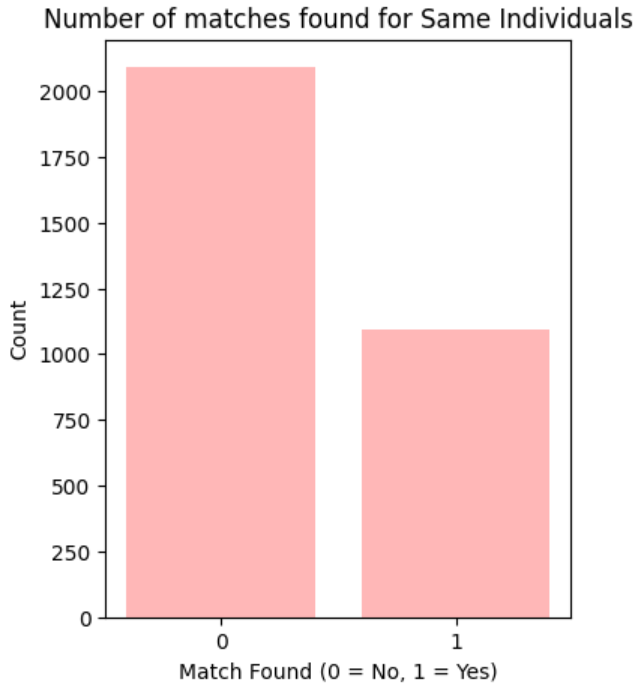
\includegraphics[width=\linewidth,height=7cm,keepaspectratio]{latex-img/d1same.png}
            \caption{Count of the number of matches for Same, Aligned Biometric Samples with Single Index Hashing and Binary PostHash Indices}
            \label{mu_same}
        \end{minipage}
        \hfill
        \begin{minipage}[b]{0.48\linewidth}
            \centering
            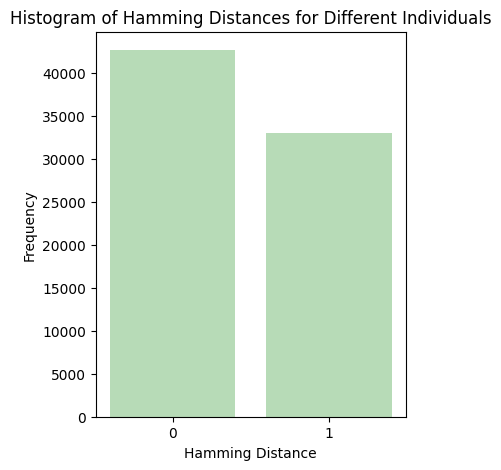
\includegraphics[width=\linewidth,height=7cm,keepaspectratio]{latex-img/d1diff.png}
            \caption{Count of the number of matches for Different, Aligned Biometric Samples with Single Index Hashing and Binary PostHash Indices}
            \label{mu_diff}
        \end{minipage}
    \end{figure}
    
    \item \text{\(d = 2\) and \(m = 1\)}: Single-index outputs (\(m=1\)) and quaternary postHash indices (\(d=2\)).
    \begin{itemize}
        \item \(q_{same}^{obs} = 42.62\%\)
        \item \(q_{diff}^{obs} = 29.84\%\)
    \end{itemize}

    \begin{figure}[H]
        \centering
        \begin{minipage}[b]{0.48\linewidth}
            \centering
            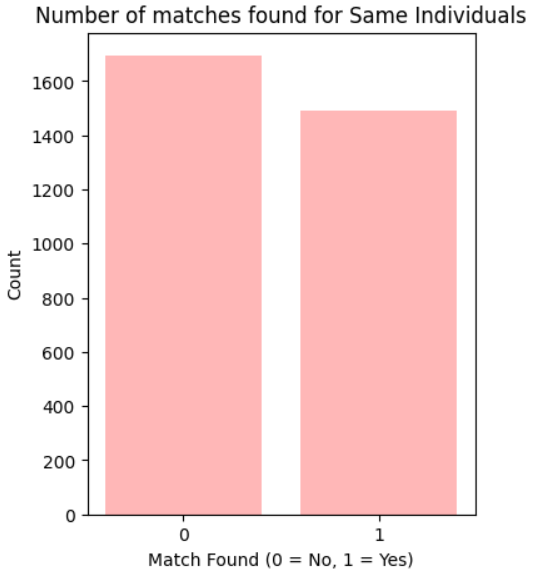
\includegraphics[width=\linewidth,height=7cm,keepaspectratio]{latex-img/d2same.png}
            \caption{Count of the number of matches for Same, Aligned Biometric Samples with Single Index Hashing and Quaternary PostHash Indices}
            \label{mu_same}
        \end{minipage}
        \hfill
        \begin{minipage}[b]{0.48\linewidth}
            \centering
            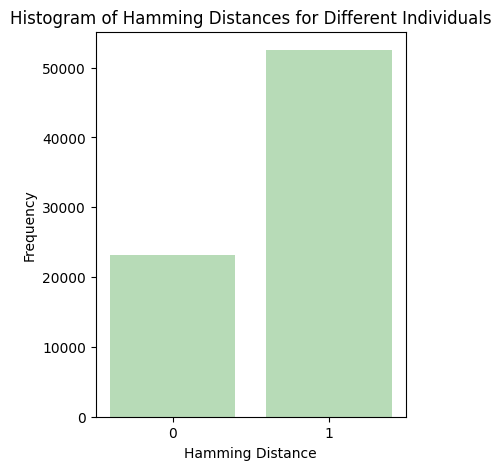
\includegraphics[width=\linewidth,height=7cm,keepaspectratio]{latex-img/d2diff.png}
            \caption{Count of the number of matches for Different, Aligned Biometric Samples with Single Index Hashing and Quaternary PostHash Indices}
            \label{mu_diff}
        \end{minipage}
    \end{figure}
    
    \item \text{\(d = 3\) and \(m = 1\)}: Single-index outputs (\(m=1\)) and octal postHash indices (\(d=3\)).
    \begin{itemize}
        \item \(q_{same}^{obs} = 32.57\%\)
        \item \(q_{diff}^{obs} = 19.04\%\)
    \end{itemize}

    \begin{figure}[H]
        \centering
        \begin{minipage}[b]{0.48\linewidth}
            \centering
            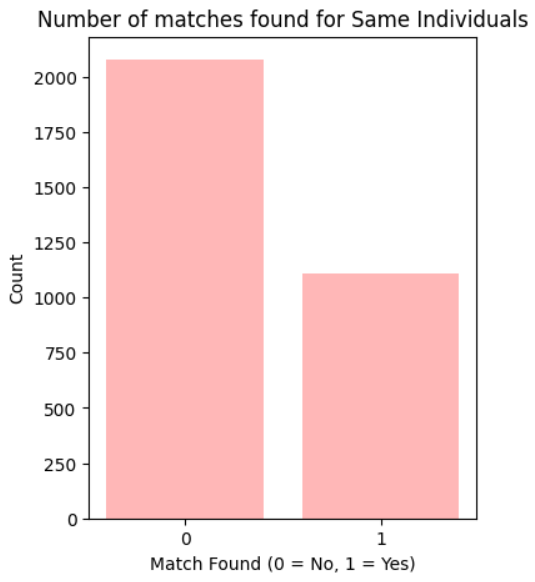
\includegraphics[width=\linewidth,height=7cm,keepaspectratio]{latex-img/d3same.png}
            \caption{Count of the number of matches for Same, Aligned Biometric Samples with Single Index Hashing and Octal PostHash Indices}
            \label{mu_same}
        \end{minipage}
        \hfill
        \begin{minipage}[b]{0.48\linewidth}
            \centering
            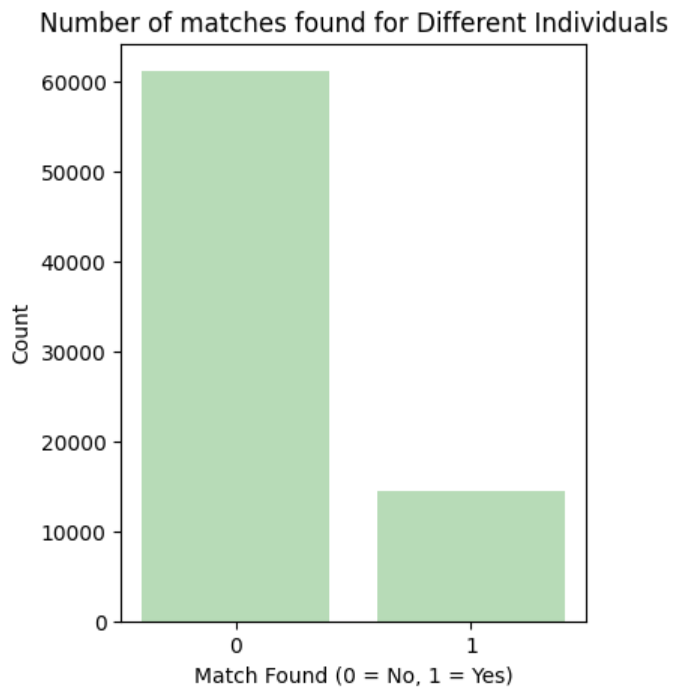
\includegraphics[width=\linewidth,height=7cm,keepaspectratio]{latex-img/d3diff.png}
            \caption{Count of the number of matches for Different, Aligned Biometric Samples with Single Index Hashing and Octal PostHash Indices}
            \label{mu_diff}
        \end{minipage}
    \end{figure}
    
    \item \text{\(d = 4\) and \(m = 1\)}: Single-index outputs (\(m=1\)) and hexa-decimal postHash indices (\(d=4\)).
    \begin{itemize}
        \item \(q_{same}^{obs} = 26.92\%\)
        \item \(q_{diff}^{obs} = 13.13\%\)
    \end{itemize}

    \begin{figure}[H]
        \centering
        \begin{minipage}[b]{0.48\linewidth}
            \centering
            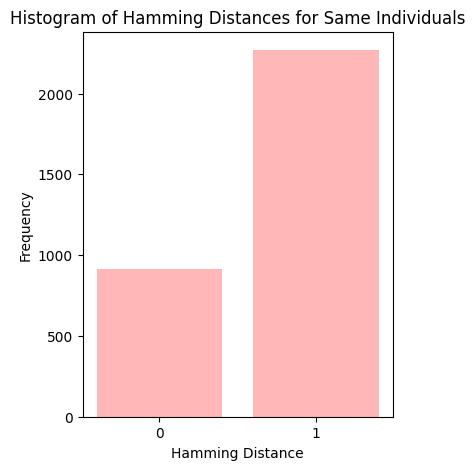
\includegraphics[width=\linewidth,height=7cm,keepaspectratio]{latex-img/d4same.png}
            \caption{Count of the number of matches for Same, Aligned Biometric Samples with Single Index Hashing and Hexa-Decimal PostHash Indices}
            \label{mu_same}
        \end{minipage}
        \hfill
        \begin{minipage}[b]{0.48\linewidth}
            \centering
            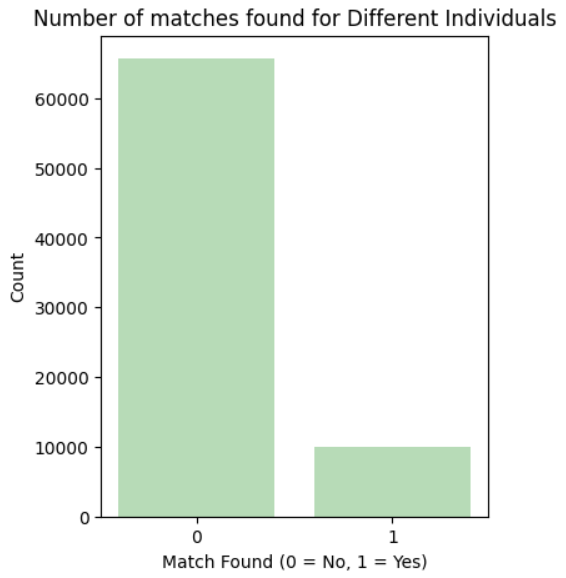
\includegraphics[width=\linewidth,height=7cm,keepaspectratio]{latex-img/d4diff.png}
            \caption{Count of the number of matches for Different, Aligned Biometric Samples with Single Index Hashing and Hexa-Decimal PostHash Indices}
            \label{mu_diff}
        \end{minipage}
    \end{figure}
\end{enumerate}

The theoretical values for \(q_{same}\) presented in Table~\ref{tab:theoretical_q} are accurate approximations, as the experimental results closely match these values. The greater discrepancy between theoretical and experimental values for \(q_{diff}\) compared to \(q_{same}\) can be attributed to the following factor: Different biometric samples exhibit higher variability, leading to a broader range of feature differences, which can cause deviations from theoretical assumptions. Outliers and noise further exacerbate the discrepancies for \(q_{diff}\). Moreover, the theoretical values for the parameter combination \(m=1\) and \(d=4\) (last row of Table~\ref{tab:theoretical_q}) align almost perfectly with the experimental results, with \(q_{same}\) values being identical and \(q_{diff}\) values differing by only approximately 0.8\%. The lookup table used for this experiment was generated using Equation~\ref{eq:GeomFormula}, followed by a redistribution of the indices across each bucket to achieve a more uniform distribution. This redistribution process was also applied to the experiment with \(d = 3\), achieving experimental results much closer to the theoretical predictions. However, this redistribution was not applied to the first three experiments, which could explain why their results show greater discrepancies.





\section{Private and Compact Biometric Matching}
% p = probability of a vein pixel being present in a given biometric sample
% delta = probability of differences between two biometric samples 
% mu = theoretical matching probability under optimal conditions (mu depends on p and delta)

\subsection{Analyzing FPR and FNR}
\section{[1:N] Matching and System Evaluation}

\subsection{Implementation of [1:N] Matching}
\subsection{System Performance Evaluation}

\newpage
\newpage
\section{Application: Private and Compact Biometric Matching}
\label{Application: Private and Compact Biometric Matching}

This section delves into the practical application of fuzzy hashing within the realm of biometric matching. Employing the Hamming distance for biometric matching offers a systematic approach by iteratively generating \textit{l} iterations of the \textit{PreHash} function, defined as:

\begin{equation}
    \begin{aligned}
        Hash_{\text{key}}^m &= Hash_{\text{key}_1, \ldots, \text{key}_l}^m(X)\\
        &= (PreHash_{\text{key}_1}^m(X), \ldots, PreHash_{\text{key}_l}^m(X))
    \end{aligned}
\end{equation}

Subsequently, the Hamming distance between the resulting hash values of two biometric samples \(X\) and \(Y\) is calculated as:

\[d_H(Hash_{key}(X), Hash_{key}(Y)) = \# \{i: PreHash_{key_i}(X) \neq PreHash_{key_i}(Y)\}\]

This expression quantifies the instances "i" where the outputs of the \textit{PreHash} function differ between samples \(X\) and \(Y\).

One notable advantage of this approach is the reduction in size of the stored biometric template. Rather than storing \textit{n} pixels, \textit{ml} integers are stored. Additionally, the key renders the reference \textit{PreHash} less privacy-sensitive compared to a biometric template. Specifically, if the key is known, each integer in the hash discloses about \(\frac{1}{p}\) pixels, revealing \(\frac{ml}{p}\) pixels at worst. This disclosure occurs because, with the keys, the hash values can potentially be reverse-engineered to reveal characteristics of the original biometric pattern. The term \(p\)​ reflects the information entropy associated with each bit being a vein (\('1'\)) and thus quantifies the average information content each disclosed pixel conveys when the hash is decoded.

Similarly, when employing the Hamming distance for biometric matching through the iterative generation of \textit{l} iterations of the \textit{PostHash} function, analogous advantages arise. Here, the stored biometric template is condensed to \textit{mld} integers instead of \textit{n} pixels. Furthermore, the key diminishes the sensitivity of the reference \textit{PostHash} in terms of privacy, exposing \(\frac{mld}{p}\) pixels at most if known. Additionally, \textit{PostHash} contributes to leakage reduction.

It's crucial to note that for both scenarios, additional privacy safeguards can be implemented, for instance a restricted access to the key. Hence, the intricacies of the biometric infrastructure must be addressed on a case-by-case basis.

\subsection{Theoretical Foundations of FPR and FNR within Fuzzy Hashing Systems}

Transforming biometric data into a hash, using methods like \textit{PreHash} or its more compact version, \textit{PostHash}, plays a key role in enhancing the system's efficiency and security. This process helps protect privacy, which in turn influences important aspects of the system's performance, such as the \hyperref[def:FNR]{False Negative Rate (FNR)} and the \hyperref[def:FPR]{False Positive Rate (FPR)}. By converting detailed biometric data into a simpler, hashed format, the system not only uses storage space more efficiently but also reduces the chances of unauthorized access to sensitive information. This transformation is crucial for maintaining the integrity of the data and provides a strong line of defense against potential security threats. Additionally, choosing the right techniques for generating these hashes can greatly improve the system's ability to distinguish between authorized and unauthorized users. This means fewer mistakes in the form of false rejections or acceptances, leading to a more accurate and dependable biometric verification process.

We establish a threshold \(t\) to evaluate the match between two biometric samples, \(X\) and \(Y\), by analyzing the Hamming distance between their hash values.
We define that a match is confirmed if the difference between \(l\) (the total iterations) and the Hamming distance is equal to or exceeds the threshold \(t\), expressed as: \[l - d_H(Hash_{\text{key}}(X), Hash_{\text{key}}(Y)) \geq t\]
In contrast, we define there being no match if the following equation holds: \[l - d_H(Hash_{\text{key}}(X), Hash_{\text{key}}(Y)) < t\]

To further refine our understanding, we use statistical methods to approximate this comparison to a normal distribution, allowing us to more accurately calculate the False Negative Rate (FNR). This measure helps us assess how often the system incorrectly fails to recognize a match between the biometric samples when there actually is one. We define:

\begin{equation}
    \label{eq:fnr}
    FNR = \Phi\left( \frac{t - l\mu_{\text{same}}^m}{\sqrt{l\mu_{\text{same}}^m}} \right)
\end{equation}

Here, \(\Phi\) denotes the Cumulative Distribution Function (CDF) of the standard normal distribution, denoted as \(\mathcal{N}(0, 1)\).

In contrast, the False Positive Rate (FPR), the proportion of non-matching biometric samples incorrectly identified as matches by the system, is defined as:

\begin{equation}
    \label{eq:fpr}
    FPR = \Phi\left(- \frac{t - l\mu_{\text{diff}}^m}{\sqrt{l\mu_{\text{diff}}^m}} \right)
\end{equation}

These formulations allow for the evaluation of false match rates based on the standard deviation and mean of the distributions for same and different samples, respectively. The upper bound \(\mu_{same}\) and \(\mu_{diff}\) are defined in Equation \ref{eq:mu}.

For instance, employing \(\Phi(-2.33) \approx 1\%\) as a benchmark, we calculate the threshold (\(t\)) from parameters \(m\) and \(l\) to achieve an FNR of 1\% and an FPR \(\leq 2^{-36} \). The resulting set of parameters is as follows: 

\begin{table}[htbp] 
    \centering
    \begin{tabular}{|c|c|c|c|c|c|c|}
        \hline
        \textit{m} & \textit{l} & \textit{t} & \textit{l}\(\mu_{\text{same}}^m\) & \textit{l}\(\mu_{\text{diff}}^m\) & \textit{FNR} & \textit{FPR} \\
        \hline
        1 & 637 & 118 & 146.6 & 49.2 & 1\% & \(2^{-37}\) \\
        2 & 961 & 34 & 50.0 & 5.7 & 1\% & \(2^{-38}\) \\
        3 & 2569 & 18 & 31.3 & 1.2 & 1\% & \(2^{-41}\) \\
        4 & 8481 & 12 & 23.8 & 0.3 & 1\% & \(2^{-43}\) \\
        5 & 32 999 & 11 & 21.3 & 0.1 & 1\% & \(2^{-51}\) \\
        6 & 140 090 & 10 & 20.8 & 0.0 & 1\% & \(2^{-67}\) \\
        7 & 568 315 & 9 & 19.5 & 0.0 & 1\% & \(2^{-51}\) \\
        8 & 2 841 573 & 11 & 22.4 & 0.0 & 1\% & \(2^{-120}\) \\
        \hline
    \end{tabular}
    \caption{Parameterization Results for FNR and FPR Calculation}
    \label{tab:parameterization}
\end{table}



\subsection{Experimental Derivation of the FPR and FNR for \(m = 1\) and \(d = 4\)}
In this subsection, we will experimentally evaluate the False Positive Rate (FPR) using compression techniques implemented through \textit{PostHash}, specifically compressing to \(D = 16\) (\(d=4\)). The introduction of compression slightly modifies the equations for false positive and false negative rates (Equations \ref{eq:fnr} and \ref{eq:fpr}), necessitating the use of \(q\) in place of \(\mu^m\). Our methodology involves processing our image dataset through a pipeline that initially applies \textit{PreHash} to generate a single index hash (\(m=1\)) for each of the \(l=637\) iterations. Subsequently, \textit{PostHash} compresses these indexes into 4-bit integers. We then compute the normalized Hamming distance between each image pair, with each image represented by \(l \times d\) bits. Lastly, we determine matches based on a specific threshold (\(t\)) tailored to the combined parameters of \(m=1\) and \(l=637\). To facilitate this experiment, we will derive the threshold \(t\) accordingly.
\section{Conclusion}
In this report, we have explored the application of fuzzy hashing to finger-vein biometric authentication, aiming to enhance both security and efficiency. Our investigation included the development and assessment of both the preHash and postHash algorithms, which transform biometric data into secure hash values that maintain consistency despite slight variations in the input data. Got it. The results of the experiments conducted throughout our project generally aligned well with the predicted values. However, as detailed in Section~\ref{sec:Application: Private and Compact Biometric Matching}, some discrepancies arose because certain assumptions of independence may not have been accurate. To address this, we modified our preHash algorithm to ensure that no vein pixel was repeated across the \(l\) iterations of preHash, and performed the first experiment from Table~\ref{tab:theoretical_parameterization_PreHash} using this new algorithm implementation. Despite these efforts, the results did not improve. This could be due to potential errors in the algorithmic implementation, or it may indicate that the chosen approach was not optimal.


\subsection{Challenges and Future Directions}
Throughout our work on this project, we encountered numerous challenges. The first significant difficulty was integrating and building upon the work of previous students. Understanding previously written code can be extremely challenging, highlighting the crucial importance of thorough documentation. We wrote a substantial amount of code for our project, ranging from algorithms such as preHash and postHash to various experimental procedures. Given the initial struggle to comprehend the existing codebase, we prioritized documenting our contributions meticulously. This included adding detailed comments and enhancing the README file to ensure clarity and ease of understanding for future developers. We believe that the comprehensive documentation we have provided will significantly benefit anyone who continues to work on this project, ensuring that our code is accessible and easy to understand.

Another significant challenge was running the experiments. With a dataset of 800 images, each experiment generated four populations of results:

- Population I: Comparisons between same biometric subjects taken from camera 1 (\(1'591\) comparisons).\\
- Population III: Comparisons between same biometric subjects taken from camera 2 (\(1'591\) comparisons).\\
- Population II: Comparisons between different biometric subjects taken from camera 1 (\(37'809\) comparisons).\\
- Population IV: Comparisons between different biometric subjects taken from camera 2 (\(37'809\) comparisons).

This amounted to a total of 78,800 comparisons per experiment, making the runtime extremely long and we spent alot of time waiting for results. We should have addressed this issue earlier but only realized the severity of the runtime problem when conducting experiments for Section~\ref{Application: Private and Compact Biometric Matching}. The extended runtime for multiple iterations of preHash and postHash combinations for each image highlighted the inefficiency. To tackle this, we revisited the previously developed pipeline code and implemented parallel processing. Additionally, we gained access to more powerful ressources (SCITAS\cite{ref4}) to run our code more efficiently. These changes drastically reduced the runtime: experiments that previously took over 24 hours to complete were reduced to just 1 hour.

However, it's important to note that despite the improved runtime, the experiments still consume a lot of resources. Some experiments, such as the last few rows of Table~\ref{tab:theoretical_parameterization_PreHash}, still take between 1 and 4 days to run. This issue can only be further addressed by refining the actual pipeline, specifically the extraction of feature vectors, and by converting the code, which is currently written in Python, to a lower-level language. This transition would likely result in more efficient code execution and reduced resource consumption. The current system requires this especially because future work will be working on a concept called "1:N matching", which adds another layer of complexity to the system, as this process involves comparing a single biometirc input against a database of multiple potential matches to identify the closest match or matches accurately.
\section{Definitions}
\begin{description}
    \item[Equal Error Rate (EER)] \label{def:EER} Metric used to evaluate the performance of a system. It represents the point at which the system's \hyperref[def:FAR]{false acceptance rate (FAR)} equals its \hyperref[def:FRR]{false rejection rate (FRR)}. A lower EER indicates a more accurate and reliable system as it signifies a balanced trade-off between security (minimizing FAR) and usability (minimizing FRR)

    \item[False Acceptance Rate (FAR)] \label{def:FAR} This is the probability of incorrectly accepting an unauthorized user

    \item[False rejection Rate (FRR)] \label{def:FRR} This is the the probability of incorrectly rejecting an authorized user

    \item[Hash Function] \label{def:Hash_Function} A hash function is an algorithm that converts input data of any size to a smaller fixed-size string of characters, which typically acts as a data fingerprint. The output, known as a hash, is unique for different inputs in ideal cases, making hash functions crucial for cryptography, data integrity, and indexing in databases.

    \item[Fuzzy Extractors] \label{def:Fuzzy_Extractors} Fuzzy extractors are cryptographic tools designed to reliably and securely generate a consistent, reproducible cryptographic key from biometric data or other noisy inputs that are inherently inconsistent. They enable the extraction of a stable key from an input that may vary slightly over different measurements, ensuring that even with minor variations, the same key can be reliably regenerated. This process typically involves two main components: a generator that produces a stable key and some public data from an initial input, and a reproducer that can regenerate the original key from a similar but not identical input using the public data.
\end{description}


\newpage
\printbibliography[heading=bibintoc, title={References}]

\end{document}

